\documentclass[14pt, a4paper]{extarticle}

\usepackage[T2A]{fontenc}
\usepackage[utf8]{inputenc}
\usepackage[english,russian]{babel}
\usepackage{url}
%\usepackage{pscyr}

%\renewcommand{\rmdefault}{ftm}
\usepackage{setspace}
\onehalfspacing

\usepackage{changepage}
\usepackage{indentfirst} %первый абзац
\usepackage[noend]{algorithmic}
\usepackage{amssymb, multicol,amsthm}
\usepackage{amsmath}
\usepackage{tabularx}
\usepackage{enumitem, multicol}
\usepackage{titleps,lipsum}
\usepackage{mathrsfs}
\usepackage{verbatim}
\usepackage{pb-diagram}
\usepackage{graphicx}
\graphicspath{ {images/} }
\usepackage{wrapfig}
%\usepackage{xcolor}
%\definecolor{new}{RGB}{255,184,92}
%\definecolor{news}{RGB}{112,112,112}
\usepackage{wallpaper}
\usepackage{float}
%\usepackage{hyperref}
%\hypersetup{
%linkbordercolor=new,
%}

%\usepackage{geometry}
%\geometry{top=3cm,bottom=2cm,left=2cm,right=2cm}

\usepackage[margin=2cm,left=3cm,right=1.5cm]{geometry}


\binoppenalty=5000
\parindent=0pt

\renewcommand{\div}{\operatorname{div}}
\newcommand{\sign}{\operatorname{sign}}
\newcommand{\grad}{\operatorname{grad}}
\newcommand{\rot}{\operatorname{rot}}
\newcommand{\const}{\operatorname{const}}
\newcommand{\diag}{\operatorname{diag}}
\renewcommand{\leq}{\leqslant}
\renewcommand{\geq}{\geqslant}
\newtheorem{State}{Утверждение}
\def\proofname{Доказательство}
\newcommand{\pd}[2]{\frac{\partial #1}{\partial #2}} 




\begin{document}

\begin{titlepage}

\begin{center}
	Министерство образования и науки Российской Федерации
	
	Федеральное государственное автономное образовательное\\[-6pt]
	учреждение высшего профессионального образования\\[-6pt]
	«Московский физико-технический институт\\[-6pt]
	(государственный университет)»
	
	Факультет управления и прикладной математики\\[-6pt]
	Кафедра вычислительных технологий и моделирования\\[-6pt]
в геофизике и биоматематике\\
\end{center}

\vspace{20mm}

\begin{center}
	{\Large {\bf Моделирование F слоя Земной ионосферы\\[8mm] }} 
	(магистерская диссертация)\\
	Направление подготовки: 03.04.01 Прикладные математика и физика
\end{center}

\vspace{20mm}

\begin{flushleft}
	\begin{tabularx}{\textwidth}{lcl}
		Выполнил: \\
		Студент 371 группы  & \raisebox{-3pt}{\rule{3cm}{0.5pt}} & Останин Павел Антонович \\[5mm]
		
		Научный руководитель:\\
		канд. физ.-мат. наук & \raisebox{-3pt}{\rule{3cm}{0.5pt}} & Кулямин Дмитрий Вячеславович \\[5mm]
	\end{tabularx}
\end{flushleft}

\vfill

\begin{center}
	Москва 2019
\end{center}

\end{titlepage}


\tableofcontents
\clearpage

\section{Введение}
%\addcontentsline{toc}{section}{Введение}
Наблюдаемый в последнее десятилетие в мировом научном сообществе переход от климатических моделей к моделям Земной системы подразумевает включение в современные модели климата и общей циркуляции атмосферы новых областей околоземного пространства, в том числе верхних слоев атмосферы (до высот порядка 500 км, когда еще уравнения гидродинамики можно считать пригодными) и моделей ионосферы. В рамках этого направления, разработка такой модели Земной системы, включающей термосферу и ионосферу, представляет собой сложную междисциплинарную проблему. Появление таких моделей является важным шагом не только для моделирования климата, но и для целого ряда самостоятельных задач, поскольку проблема описания и прогноза ионосферы важна не столько с точки зрения ее взаимодействия с нейтральной атмосферой и возможным влиянием на климатические характеристики атмосферы, но с прикладным значением этой среды. 

Точная информация о состоянии системы термосфера-ионосфера требуется для решения ряда задач космической отрасли, межконтинентальной и спутниковой радиокоммуникации, а также радиолокации, поскольку оно частично определяет характеристики движения низкоорбитальных спутников, а также условия для распространения радиосигналов, обеспечивающих работу систем дальней радиосвязи, радиолокации, а также навигационных систем глобального спутникового позиционирования (GPS и российскую ГЛОНАСС). Таким образом, исследование и прогноз глобального состояния ионосферы в практическом смысле наиболее важны для развития технологий высокоточной навигации, повышения надежности и достоверности работы систем связи и других прикладных задач. 

Проблема описания характеристик Земной ионосферы и термосферы традиционно решается на основе обработки имеющихся экспериментальных аэрономических, динамических, радиофизических и других типов данных с построением эмпирических моделей. Созданные таким образом эмпирические модели верхней атмосферы в своей основе являются климатологией глобального состояния в определенных условиях и по большей части не учитывают изменчивость среды, вызванную как внешними, так и внутренними факторами (такими как нелинейные волновые процессы в термосфере и ионосфере и т.~п.). В то же время эти модели широко применяются для решения важных прикладных задач. Примерами таких справочных моделей являются модели ионосферы IRI, SIMP и др. [1,2]. На сегодняшний день общее количество и уровень развития численных моделей верхней атмосферы ниже по сравнению с моделями прогноза погоды и климата для нижних слоев атмосферы. 

Наиболее развитые модели ионосферы, применяемые в том числе для прогностических целей, разрабатываются в основном в крупных центрах и консорциумах различных институтов. К таковым можно отнести следующие современные совместные модели термосферы и ионосферы: американские модели NCAR TIEGCM, TIEM-GCM [3]; английские модели UCL CTIP-CMAT [4]; отечественные модели UAM [5], GCM-TIP [6]. К аналогичным более комплексным моделям можно отнести развиваемые в последние годы модели всей атмосферы (для высот от 0 до 500 км и более), в основном создаваемые для решения проблем учета взаимодействия нижних и верхних слоев: модели WACCM [7] в различных версиях (включает TIEGCM [3]), IDEA и WAM (включает CTIP и др.) [8]. Разработки таких комплексных моделей, включающих разные слои атмосферы, даже в ведущих мировых центрах находятся фактически на начальных этапах.

Известно, что проблемы описания процессов формирования нижних слоев ионосферы (D, E слои, высоты 60-130 км) и верхних слоев (F слой, высоты 130-600 км) существенно различаются: в нижних слоях ионосферы при низкой концентрации ионов собственной динамикой ионов можно пренебречь (ионы переносятся нейтральным ветром, при этом ключевыми процессами являются ионизация и химические взаимодействия), однако процессы, связанные с ионизацией нейтральной атмосферы в этих областях, сложны. В верхних слоях ионосферы ситуация иная: концентрация ионов относительно высока, вследствие чего ключевыми становятся динамические свойства плазмы и ее взаимодействие с магнитными и электрическими полями, а учет процессов динамического взаимодействия ионов с нейтральной атмосферой является непременным условием правильной постановки задачи, в то же время описание процессов ионизации нейтральной атмосферы много проще, чем в нижних слоях. Поскольку динамические свойства плазмы, перенос ионов и электронов, а также роль электромагнитных сил в верхних слоях ионосферы важны, то, следовательно, важно и описание магнитного поля Земли. 

Целью настоящей работы является описание создаваемой в ИВМ РАН динамической модели F слоя ионосферы. Основное содержание работы включает формулирование полной системы уравнений модели и описание метода ее решения. Данная работа проводится в рамках решения общей задачи создания глобальной динамической совместной модели термосферы-ионосферы ИВМ РАН (для высот 90-500 км) на основе представленной модели ионосферы с включением ее в качестве согласованного вычислительного блока в созданную ранее модель общей циркуляции термосферы [9]. Перспективной целью разработок моделей верхней атмосферы ИВМ РАН является создание модели Земной системы, включающей согласованное описание всех ключевых слоев атмосферы (для высот 0-500 км). В основе данной модели предполагается соединение в области нижней термосферы разработанных совместных моделей нижней атмосферы и ионосферы (до высот 90-130 км) [10] и разрабатываемой в настоящее время модели термосферы-ионосферы Земли (высотная область 100-500 км).

Одной из ключевых задач применения данной модели является прогноз глобального состояния Земной ионосферы. Для решения данной задачи предполагается создание специализированной для Земной ионосферы системы усвоения данных наблюдений на основе данной модели с использованием разработанной в ИВМ РАН методологии [11]. Поскольку предлагаемая методология разработана с учетом использования метода расщепления, при разработке модели ионосферы, представленной в данной работе, этот метод предполагается основным.


\section{Модель ионосферы}
\sectionmark{Модель ионосферы}
%\addcontentsline{toc}{section}{Модель ионосферы}

\subsection{Вывод используемых уравнений}
\subsectionmark{Вывод используемых уравнений}

Ионосфера~---~это ионизованная часть верхней атмосферы, приблизительно от 60~км до 1000~км, целиком окружающая Землю. Основной источник плазмы~---~фотоионизация нейтральных молекул под действием солнечного ультрафиолета и рентгеновского излучения. Ионы вступают в химические реакции с нейтральными молекулами, рекомбинируют с электронами и диффундируют в другие высоты или перемещаются нейтральным ветром. Но диффузия и перенос подвержены влиянию собственного магнитного поля Земли.

\medskip

В рассматриваемом приближении моделируется эволюция концентрации $n_e$ электронов во времени и пространстве в верхней ионосфере (в F-слое).

\medskip

В модели решается уравнение неразрывности для глобального поля концентрации свободных зарядов в области высот (100-500 км)

\begin{equation}
\dfrac{\partial n_i}{\partial t} + \nabla \left(n_i \vec{u}_i\right) = \dfrac{\delta n_i}{\delta t} = R_i.
\label{continuity_eq}
\end{equation}

Здесь введены обозначения: $n_i$~---~концентрация ионов, $\vec{u}_i$~---~средняя скорость переноса ионов. В правой части учитываются столкновительные члены, источники (главным образом ионизация солнечным излучением) и стоки.

Представленная в работе модель ионосферы основывается на следующих приближениях: отдельно рассматривается F слой ионосферы Земли, как зона максимального по величине содержания электронов и ионов в атмосфере, а также как ключевая область практического интереса (вследствие определения им максимальной критической частоты отражения радиосигналов по концентрации электронов на пике F слоя, а также наиболее значительной доли содержания общего количества электронов); из-за фотохимического преобладания ионизации атомарного кислорода O и рекомбинации его иона O$^+$ с основными составляющими O$_2$ и N$_2$ на этих высотах используется одноионная формулировка модели; предполагается локальная квазинейтральность плазмы ($n_e = n_i$); считается, что движение электронов и ионов происходит совместно вдоль силовых линий магнитного поля Земли; предполагается преобладание в динамике ионосферной плазмы амбиполярной диффузии вдоль силовых линий; используется дипольное приближения формы магнитного поля Земли.


Здесь  $p_e = n_e k T_e$, $p_i = n_i k T_i$~---~парциальные давления электронного и ионного газов соответственно, полученные из уравнения состояния для приближений идеального газа, а $T_e$, $T_i$~---~соответствующие температуры для каждой компоненты плазмы, $\nu_{in}$~---~частота ион-нейтральных столкновений, $\vec{u}$~---~скорость движения нейтралов, $\vec{E}$~---~внешние электрические поля, $\vec{B}$~---~магнитное поле Земли, $e$~---~заряд электрона, $m_i$~---~масса иона.

%%%%%%%%%%%%%%%%%%%%%%%%%%%%%%%%%%%



Считаем $n_e=n_i = n(O^+)$, т.~е. рассматриваем только электроны и ионы кислорода (в F-слое больше всего ионов $O^+$), а плазму считаем квазинейтральной. Последнее условие позволяет записать уравнение неразрывности для $n_i$ в том же виде, что и для электронной концентрации.

\medskip

За динамику в верхней атмосфере в рассматриваемой модели отвечает амбиполярная диффузия. Её суть заключается в следующем: масса электрона гораздо меньше, чем масса иона кислорода, вследствие чего электроны и ионы разделяются пространственно. Вследствие этого разделяются и заряды, и возникает добавочное электрическое поле. Это поле препятствует дальнейшему разделению слоёв. После его создания электроны и ионы движутся как единый газ.

Для вывода уравнения амбиполярной диффузии используем общее уравнение движения в следующей форме: 
\begin{gather} 
nm\dfrac{D\vec{u}}{Dt}+\vec{\nabla} p + \vec{\nabla}\cdot \hat{\tau} - ne(\vec{E}+\vec{u}\times \vec{B})+nm[-\vec{G}+2\vec{\Omega}\times \vec{u}+\vec{\Omega}\times(\vec{\Omega}\times\vec{r})]=\nonumber\\
=\sum_t nm\nu_t (\vec{u}_t-\vec{u})+ \vec{f}(\vec{q}).
\end{gather}
В этом уравнении $\dfrac{D}{Dt}=\dfrac{\partial}{\partial t}+(\vec{u}; \vec{\nabla})\vec{u}$~---~полная производная; $u$~---~скорость диффузии; $n$~---~концентрация электронов; $m$~---~масса электрона; $\hat{\tau}$~---~тензор напряжений; $\vec{G}$~---~ускорение свободного падения; в квадратных скобках помимо $\vec{G}$ стоят слагаемые, связанные с неинерциальностью системы отсчета, вызванной вращением Земли с угловой скоростью $\vec{\Omega}$; в правой части сумма отвечает за столкновения электронов с различными частицами (разные типы частиц нумеруются индексом $t$), а последнее слагаемое зависит от тепловых потоков, которые в частично ионизованной плазме малы и отбрасываются. Уравнение записано в системе координат, связанной с Землёй.

\bigskip

Далее используем т.~н. диффузионную аппроксимацию: отбросим всю полную производную в силу её малости по сравнению с градиентом давления:

\begin{itemize}

\item[•] $\dfrac{|nm(\vec{u}; \vec{\nabla})\vec{u}|}{|\vec{\nabla}p|}\approx \dfrac{nmu^2/L}{nkT}\approx \dfrac{u^2}{kT/m}=M^2$~---~квадрат числа Маха. При малых числах Маха (т.~е. при дозвуковых течениях) первое слагаемое можно отбросить.

\item[•] $\dfrac{|nm\partial\vec{u}/\partial t|)\vec{u}}{|\vec{\nabla}p|}\approx \dfrac{L}{\tau} \dfrac{u}{kT/m}\approx M\dfrac{L/\tau}{\sqrt{kT/m}}$, где $\tau$ и $L$~---~характерное время процессов в плазме и характерный размер области, в которой находится рассматриваемая часть плазмы.

\end{itemize}

Для медленно меняющихся и дозвуковых потоков диффузионная аппроксимация применима.

\bigskip

Помимо квазинейтральности ($n_e=n_i$) предполагаем движение электронов с ионами единым целым: $n_e \vec{u}_e=n_i \vec{u}_i$. Отбросим также и слагаемые, связанные с неинерциальностью системы отсчета в предположении их малости в сравнении с силами тяжести и магнитными силами.

Как уже упоминалось выше, считаем, что имеются ионы всего одного вида~---~кислорода. Это справедливо в рассматриваемом F-слое (выше $\approx 130$~км и до $1000$~км).

Запишем в приведенных приближениях общее уравнение движения для электронов и ионов в проекциях на магнитные силовые линии (индекс $\parallel$ указывает соответствующую проекцию):

\begin{equation}
\begin{cases}
\vec{\nabla}_\parallel p_i + (\vec{\nabla}\cdot \hat{\tau}_i)_\parallel + n_ie\vec{E}_\parallel-n_im_i\vec{G}_\parallel=\\
\textrm{ }\textrm{ }\textrm{ }\textrm{ }\textrm{ }=n_im_i\nu_{ie}(\vec{u}_e-\vec{u}_i)_\parallel+n_im_i\nu_{in}(\vec{u}_n-\vec{u}_i)_\parallel\\
\vec{\nabla}_\parallel p_e + (\vec{\nabla}\cdot \hat{\tau}_e)_\parallel - n_ee\vec{E}_\parallel-n_em_e\vec{G}_\parallel=\\
\textrm{ }\textrm{ }\textrm{ }\textrm{ }\textrm{ }=n_em_e\nu_{ei}(\vec{u}_i-\vec{u}_e)_\parallel+n_em_e\nu_{en}(\vec{u}_n-\vec{u}_e)_\parallel
\end{cases} 
\end{equation}

Сложив эти уравнения и учтя, что $n_e=n_i$, $\vec{u}_e=\vec{u}_i$, $n_im_i\nu_{ei}=n_em_e\nu_{ei}$, получим уравнение, не содержащее электрического поля, возникшего вследствие разделения электронов и ионов по слоям:
\begin{equation}
\vec{\nabla}_\parallel (p_i+p_e) + (\vec{\nabla}\cdot (\hat{\tau}_i+\hat{\tau}_e))_\parallel-n_i(m_i+m_e)\vec{G}_\parallel=n_i(m_i\nu_{in}+m_e\nu_{en})(\vec{u}_n-\vec{u}_i)_\parallel.
\end{equation}

Теперь можно отбросить все слагаемые, содержащие массу электрона по сравнению с такими же слагаемыми, но уже с массой иона. После этого заменим давление $p_i=n_ikT_i$, $p_e=n_ikT_e$ и обозначим $T_p=\dfrac{1}{2}(T_e+T_i)$. Выразив из правой части векторную разность скоростей, получим закон амбиполярной диффузии, дающий характеристику средней скорости диффундирующих ионов: 
\begin{equation}
\vec{u}_{i\parallel} = \vec{u}_{n\parallel} - \dfrac{2kT_p}{m_i\nu_{in}}\left(\dfrac{1}{n_i}\vec{\nabla}_\parallel n_i+\dfrac{1}{T_p}\vec{\nabla}_\parallel T_p-\dfrac{m_i\vec{G}_\parallel}{2kT_p}+\dfrac{(\vec{\nabla}\cdot\hat{\tau_i})_\parallel}{2n_ikT_p}\right).
\end{equation}

Обозначим $D=\dfrac{2kT_p}{m_i\nu_{in}}$~---~коэффициент амбиполярной диффузии.

Теперь обратимся к компоненте скорости, ортогональной вектору $\vec{B}$. В соответствии с оценками, приведёнными в [], будем считать, что в плоскости, ортогональной вектору $\vec{B}$ главный процесс~---~дрейф, связанный с внешними полями (это справедливо ввиду сильной замагниченности плазмы). Тогда в проекции на плоскость, ортогональную $\vec{B}$, уравнение движения для ионов можно записать в форме 
\begin{equation}
n_ie\vec{E}_\perp + n_ie[\vec{u}_{i\perp}\times \vec{B}]=0.
\end{equation}
Домножим векторно на $\vec{B}$: $$[e\vec{E}_\perp\times\vec{B}]+e[[\vec{u}_{i\perp}\times\vec{B}]\times\vec{B}]=0\Leftrightarrow$$ $$\Leftrightarrow[e\vec{E}_\perp\times\vec{B}]-eB^2\vec{u}_{i\perp}+e(\vec{u}_{i\perp};\vec{B})\vec{B}=0.$$
Отметим также, что $\vec{E}_\perp\times \vec{B} = (\vec{E}_\perp+\vec{E}_\parallel)\times \vec{B} = \vec{E}\times\vec{B}$.

Учтём, что рассматривается компонента, ортогональная $\vec{B}$, поэтому скалярное произведение в третьем слагаемом равно нулю. Это позволяет выразить искомый вектор $\vec{u}_{i\perp}$: 
\begin{equation}
\vec{u}_{i\perp}=\dfrac{[\vec{E}\times\vec{B}]}{B^2}.
\end{equation}

После нахождения компонент $\vec{u}$, параллельной и ортогональной полю, из уравнения неразрывности окончательно получаем следующее векторное уравнение, описывающее искомую эволюцию электронной концентрации: \begin{equation}\label{general_eq}
\dfrac{\partial n_i}{\partial t} = -\div(n_i \vec{u}_{n\parallel})-\div\left(n_i\dfrac{1}{B^2}[\vec{E}\times \vec{B}] \right)+$$ $$+\div\left(D\left[\vec{\nabla}_\parallel n_i +n_i\dfrac{1}{T_p}\vec{\nabla}_\parallel T_p - \dfrac{n_i m_i}{2kT_p}\vec{g}_\parallel\right]\right)+[P-k_in_i].
\end{equation}




%%%%%%%%%%%%%%%%%%%%%%%%%%%%%%%%%%%%%

%Таким образом, выделение направления, совпадающего с магнитным полем Земли, и плоскости, перпендикулярной этому направлению, а также последующее проецирование данного векторного уравнения (\ref{amb_complete}) на данные геометрические направления, приводит к выражению для параллельной $u_\parallel$   и перпендикулярной $u_\perp$   составляющих скорости движения ионов.

%В параллельном магнитному полю Земли направлении, используя приведенный выше баланс (\ref{force_balance}), получаем <<классическое>> уравнение амбиполярной диффузии вдоль магнитных линий:

%\begin{align*}
%\nabla_\parallel(p_i+p_e) - n_im_i g_\parallel = n_i m_i \nu_{in}\left(\vec{u}-\vec{u}_i\right)_\parallel \Rightarrow \nonumber\\
%u_{i\parallel} = u_\parallel - \dfrac{1}{m_i\nu_{in}}\left(\dfrac{1}{n_i}\nabla_\parallel(p_i + p_e) - m_i g_\parallel\right) \Rightarrow \nonumber\\
%u_{i\parallel} = u_\parallel - \dfrac{k(T_i+T_e)}{m_i\nu_{in}}\left(\dfrac{1}{n_i}\nabla_\parallel(n_i) + \dfrac{1}{T_i+T_e}\nabla_\parallel(T_i+T_e) - \dfrac{m_i}{k(T_i+T_e)}g_\parallel\right)\nonumber\\
%D = \dfrac{k(T_i+T_e)}{m_i\nu_{in}}, \mbox{ } H = \dfrac{k(T_i+T_e)}{m_ig}, \mbox{ }T_p = \dfrac{1}{2} (T_i + T_e), %\label{u_par_perp}
%\end{align*}
%где $D$ и $H$~---~коэффициент амбиполярной диффузии и масштаб высоты для ионосферной плазмы соответственно.

%В поперечном направлении можно использовать баланс силы Лоренца и столкновительного члена (аналогичный применяемому нами в модели термосферы для описания ион-нейтрального взаимодействия), однако эмпирические оценки для высот F слоя ионосферы показывают, что доминирующей составляющей в поперечном направлении является электромагнитный дрейф, так что нетрудно получить $u_{i\perp} = \dfrac{1}{B^2}\left[\vec{E}_0 \times \vec{B}\right]$.

%Полученное с учетом всех приближений уравнение неразрывности для электронной концентрации в F слое ионосферы имеет вид:
%\begin{align}
%\dfrac{\partial n_i}{\partial t} = -\textrm{div}\left(n_i\vec{u}\parallel\right) - \textrm{div}\left(n_i \dfrac{1}{B^2}\left[\vec{E}'\times\vec{B}\right]_\perp\right) + \nonumber\\
%+ \textrm{div}\left(D\left(\nabla_\parallel(n_i) + n_i\dfrac{1}{T_p} \nabla_\parallel T_p - \dfrac{n_im_i}{2kT_p}\vec{g}_\parallel\right)\right) + \left[P - k_in_i\right] %%\label{continuity_eq_electron_concentration}
%\end{align}
%В этом уравнении в правой части член $P$~---~скорость ионизации солнечным излучением нейтральных составляющих термосферы (в данной модели атомарного кислорода О до иона О$^+$), $k_i$~---~суммарная %скорость рекомбинации при столкновениях с нейтралами (в данном случае учитываются столкновения только с ключевыми компонентами термосферы~---~молекулярным кислородом и азотом).


Для решения этой системы разумным представляется использование криволинейной системы координат, связанной с направлениями магнитного поля Земли (так называемых <<магнитных трубок>>), что сделано в ряде существующих в мире моделей [3-5]. Этот метод позволяет решать фактически одномерные уравнения в параллельном трубкам направлении и отдельно рассчитывать поперечное смещение трубок. Однако при реализации данного подхода возникает ряд трудностей, связанных с правильным расчетом коэффициентов Ламэ, с расчетом ключевых внешних для ионосферы параметров (в частности, распределения всех характеристик нейтральной термосферы), с расчетом температур ионов и электронов, которые главным образом привязаны к вертикальному направлению. Эти сложности накладывают существенные ограничения при разработке совместных моделей для системы термосфера-ионосфера, поскольку модели термосферы традиционно разрабатываются в географической системе координат с вертикальным направлением вдоль силы тяжести.

Поэтому в данной работе в качестве базовой системы координат для модели ионосферы взята система сферических координат в приближении тонкого сферического слоя, согласованная с постановкой модели циркуляции термосферы ИВМ РАН. Выбор данной системы обусловлен как задачей включения модели ионосферы в единую совместную с термосферой модель, так и перспективной целью разработки полной модели нейтральной атмосферы и ионосферы (от 0 до 500 км).


\subsection{Основное уравнение в сферической системе координат (в приближении тонкого сферического слоя)}
\subsectionmark{Основное уравнение в сферической системе координат}


Получим полное уравнение неразрывности с учетом трехмерного переноса плазмы при указанных выше приближениях из общего уравнения (\ref{general_eq}) в данной системе координат, которое использовано в конечном варианте модели. 


Перейдем от векторной записи уравнения неразрывности $(7)$, описывающего динамику электронной плотности, к сферическим координатам $(\lambda, \varphi, z)$, где $\lambda$~---~долгота, $\lambda \in [0, 2\pi]$, $\varphi$~---~широта, $\varphi \in \left[-\dfrac{\pi}{2};\dfrac{\pi}{2}\right]$, $z$~---~высота, отсчитываемая от радиуса Земли $a$. 

Используем приближение тонкого сферического слоя: для частных производных по $x$ и $y$ запишем формулы $$\dfrac{\partial}{\partial x}=\dfrac{1}{a\cos\varphi}\dfrac{\partial}{\partial\lambda},\mbox{ } \dfrac{\partial}{\partial y} = \dfrac{1}{a}\dfrac{\partial}{\partial\varphi},$$ в которых $a$ считаем постоянным. Для дивергенции в сферических координатах в приближении тонкого сферического слоя используем \begin{equation}\label{divergence}\div(n_i \vec{a}) = \dfrac{1}{a\cos\varphi}\left[\dfrac{\partial}{\partial\lambda}(n_i a_x)+\dfrac{\partial}{\partial\varphi}(n_i a_y\cos\varphi)\right]+\dfrac{\partial}{\partial z}(n_i a_z).\end{equation}
Для векторного поля, стоящего под общим знаком дивергенции в правой части уравнения $(7)$ введём следующие обозначения: $$\vec{\alpha}=-\vec{u}_\parallel-\dfrac{1}{B^2}[\vec{E}\times\vec{B}]; \mbox{ }\vec{\beta} = \vec{\nabla}_\parallel n_i;$$ $$\vec{\gamma} = \left(\dfrac{1}{T_p}\vec{\nabla}_\parallel  T_p - \dfrac{m_i \vec{g}_\parallel}{2kT_p}\right)=\left(\dfrac{1}{T_p}\vec{\nabla}_\parallel  T_p - \dfrac{1}{H}\dfrac{\vec{g}_\parallel}{g}\right).$$
К вектору $\vec{\alpha}$ отнесены компоненты, отвечающие переносу без диффузии, в вектор $\vec{\beta}$ вошли слагаемые с производными от $n_i$, а оставшийся вектор $\vec{\gamma}$ соответствует эффективной скорости при диффузии. Обозначим $DYZ(n_i) = \div(D\vec{\beta})$, $Tr(n_i) = \div(n_i\vec{\alpha})$, $DTr(n_i) = \div(Dn_i\vec{\gamma})$. С учетом этих обозначений уравнение $(7)$ можно переписать в виде \begin{equation}\label{main_eq}\dfrac{\partial n_i}{\partial t} = \div(n_i\vec{\alpha} + D\vec{\beta}+Dn_i\vec{\gamma})+[P-kn_i]=$$ $$=DYZ(n_i)+DTr(n_i)+Tr(n_i)+[P-kn_i]. \end{equation}
Запишем теперь введённые векторы $\vec{\alpha}, \vec{\beta}, \vec{\gamma}$ в компонентах и применим для дивергенции формулу (\ref{divergence}). 

В рассматриваемое уравнение входит вектор напряженности магнитного поля. В рассматриваемой постановке принимается дипольное приближение, в котором компоненты вектора напряженности магнитного поля выражаются через широту с помощью углов магнитного наклонения $I\approx \arctg(2\tg\varphi)$ и угла склонения $D$ по формулам
\begin{equation}\label{magn_field}\vec{B} = \left(\begin{array}{crl}
B\cos I \sin D\\
B\cos I \cos D\\
-B\sin I
\end{array}\right).\end{equation}
Кроме того, в приближении совпадения магнитных и географических полюсов $D\approx 0$, поэтому далее считается, что 

\begin{equation}\label{magn_field_approx}\vec{B}\approx
\left(\begin{array}{crl}
0\\
B\cos I\\
-B\sin I
\end{array}\right).\end{equation}


Учтём, что в приближении совпадения магнитных и географических полюсов угол магнитного наклонения $I\approx \arctg(2\tg\varphi)$. Это означает, что для некоторого вектора $\vec{a}$ его составляющая вдоль магнитного поля \begin{equation}\vec{a}_\parallel = \left(\vec{a},\dfrac{\vec{B}}{B}\right)\dfrac{\vec{B}}{B} = (a_y\cos I - a_z\sin I)\cdot \left(\begin{array}{crl}
0\\
\cos I\\
-\sin I
\end{array}\right).\end{equation}
Аналогично, для параллельной полю компоненты градиента некоторой скалярной функции $f$ можем записать \begin{equation}\vec{\nabla}_\parallel f = \left(\vec{\nabla} f,\dfrac{\vec{B}}{B}\right)\dfrac{\vec{B}}{B} = \left(\dfrac{\partial f}{\partial y}\cos I - \dfrac{\partial f}{\partial z}\sin I\right)\cdot \left(\begin{array}{crl}
0\\
\cos I\\
-\sin I
\end{array}\right).\end{equation}
С учетом этих замечаний заключаем, что вектор $\vec{\alpha}$ имеет компоненты \begin{equation}\vec{\alpha} = 
\left(\begin{array}{crl}
0\\
-u_y\cos^2 I + u_z\sin I \cos I\\
u_y\cos I \sin I - u_z\sin^2 I
\end{array}\right) - \dfrac{1}{B}
\left(\begin{array}{crl}
-E_y\sin I - E_z\cos I\\
E_x\sin I\\
E_x\cos I
\end{array}\right).\end{equation}
Вектор $\vec{\beta}$~---~параллельная полю составляющая градиента функции $n_i$, поэтому с учётом формул для $\dfrac{\partial}{\partial y}$ и $\dfrac{\partial}{\partial z}$ запишем \begin{equation}\vec{\beta} = \left(\begin{array}{crl}
0\\
\dfrac{\partial n_i}{\partial y}\cos^2 I - \dfrac{\partial n_i}{\partial z}\cos I\sin I\\
-\dfrac{\partial n_i}{\partial y}\cos I\sin I + \dfrac{\partial n_i}{\partial z}\sin^2 I
\end{array}\right) = \left(\begin{array}{crl}
0\\
\dfrac{1}{a}\dfrac{\partial n_i}{\partial \varphi}\cos^2 I - \dfrac{\partial n_i}{\partial z}\cos I\sin I\\
-\dfrac{1}{a}\dfrac{\partial n_i}{\partial \varphi}\cos I\sin I + \dfrac{\partial n_i}{\partial z}\sin^2 I
\end{array}\right)\end{equation}
Оставшийся вектор $\vec{\gamma}$~---~линейная комбинация градиента скалярной функции $T_p$ и параллельной полю компоненты вектора $\vec{g} = (0, 0, -g)^T$: \begin{equation}\vec{\gamma} = \dfrac{1}{T_p}\left(\begin{array}{crl}
0\\
\dfrac{1}{a}\dfrac{\partial T_p}{\partial \varphi}\cos^2 I - \dfrac{\partial T_p}{\partial z}\cos I\sin I\\
-\dfrac{1}{a}\dfrac{\partial T_p}{\partial \varphi}\cos I\sin I + \dfrac{\partial T_p}{\partial z}\sin^2 I
\end{array}\right) -\dfrac{1}{H} \left(\begin{array}{crl}
0\\
\sin I\cos I\\
-\sin^2 I
\end{array}\right)\end{equation}
Теперь с помощью записанной ранее формулы для дивергенции (\ref{divergence}) окончательно получаем для слагаемых в правой части уравнения (\ref{main_eq}) выражения: \begin{equation}\label{Tr} Tr(n_i) = \div (n_i\vec{\alpha}) = \dfrac{1}{a\cos\varphi}\left[\dfrac{\partial}{\partial\lambda}(n_i\alpha_x) + \dfrac{\partial}{\partial\varphi}(n_i \alpha_y\cos\varphi) \right]+\dfrac{\partial}{\partial z}(n_i \alpha_z)=$$ $$\dfrac{1}{a\cos\varphi}\dfrac{\partial}{\partial\lambda}\left[n_i\dfrac{1}{B}(E_y\sin I + E_z\cos I)\right]+\dfrac{1}{a\cos\varphi}\dfrac{\partial}{\partial\varphi}\bigg[\bigg(u_z\sin I \cos I - u_y\cos^2 I -$$ $$- \dfrac{E_x}{B}\sin I\bigg)n_i\cos\varphi\bigg]+\dfrac{\partial}{\partial z}\left[\left(u_y\cos I \sin I -u_z\sin^2 I - \dfrac{E_x}{B}\cos I\right)n_i\right];\end{equation}

\begin{equation}\label{DYZ} DYZ(n_i) = \div (D\vec{\beta}) = \dfrac{1}{a\cos\varphi}\dfrac{\partial}{\partial\varphi}\left(D\cos\varphi\left[\dfrac{1}{a}\dfrac{\partial n_i}{\partial\varphi} \cos^2 I -\dfrac{\partial n_i}{\partial z}\cos I\sin I\right]\right)+$$ $$ + \dfrac{\partial}{\partial z}\left(D\left[\dfrac{\partial n_i}{\partial z}\sin^2 I - \dfrac{1}{a}\dfrac{\partial n_i}{\partial\varphi}\cos I \sin I\right]\right);\end{equation}

\begin{equation}\label{DTr} DTr(n_i) = \div(Dn_i\vec{\gamma}) = \dfrac{1}{a\cos\varphi}\dfrac{\partial}{\partial \varphi}\bigg[\bigg(\dfrac{1}{a}\dfrac{1}{T_p}\dfrac{\partial T_p}{\partial\varphi}\cos^2 I-\dfrac{1}{T_p}\dfrac{\partial T_p}{\partial z}\cos I \sin I - $$ $$-\dfrac{1}{H}\sin I \cos I\bigg)Dn_i\cos\varphi\bigg] + \dfrac{\partial}{\partial z}\bigg[\bigg(-\dfrac{1}{a}\dfrac{1}{T_p}\dfrac{\partial T_p}{\partial \varphi}\cos I \sin I +$$ $$ +\dfrac{1}{T_p}\dfrac{\partial T_p}{\partial z}\sin^2 I+\dfrac{1}{H}\sin^2I\bigg)Dn_i\bigg].\end{equation}




%%%%%%%%%%%%%%%%%%%%%%%%%%%%%%%%%%%%%%%%%%%%%%%%%%%%%%%%%%%%%%%%%%%%%%%%%%%%%%%%%%%%%%%%







\subsection{Внешние параметры уравнения}
\subsectionmark{Внешние параметры уравнения}

Входящие в уравнение в качестве внешних параметров функции фотоионизации, рекомбинации, температуры нейтралов, электронов и ионов, а также концентрации молекул $N_2$, $O_2$ и $O$ задаются аналитическими формулами. 

Для концентраций используем Больцмановское распределение по высоте: \begin{equation} n_{O_2, N_2, O} (z)= n_{O_2, N_2, O} (z_0)\cdot \exp\left(-\dfrac{M_{O_2, N_2, O}g}{R_0T_n}(z-z_0)\right).\end{equation} Концентрации на высоте $z_0\approx 100$~км полагаем равными $n_{O_2} = 5{,}6\cdot 10^9$~см$^{-3}$, $n_{O} = 2{,}8\cdot 10^{10}$~см$^{-3}$, $n_{N_2} = 5{,}2\cdot 10^{10}$~см$^{-3}$. 

Температуры вычисляем по аналитическим формулам \begin{equation}T(z)=T_\infty - (T_\infty-T_0)\exp\left(-\dfrac{g}{RT_\infty}(z-z_0)\right),\end{equation} где $R=\dfrac{R_0}{M_{air}}\approx 287$~Дж$\cdot$кг$^{-1}\cdot$K$^{-1}$, $R_0$~---~универсальная газовая постоянная. Константы $T_\infty$ для разных составляющих приближённо считаем равными $T_{n\infty}=800$~К, $T_{i\infty}=950$~К, $T_{e\infty}=2200$~К.

Функции рекомбинации и фотоионизации (в дневное время) можно приближенно вычислять по следующим формулам: \begin{equation}P=4\cdot10^{-7}\cdot n_O(z)\textrm{ [с}^{-1}\textrm{]}\end{equation} \begin{equation}k=1{,}2\cdot10^{-12}\cdot n_{N_2}(z)+2{,}1\cdot 10^{-11}\cdot n_{O_2}(z) \textrm{ [с}^{-1}\textrm{]}.\end{equation}

При неизменных по времени функциях фотоионизации и рекомбинации $P$ и $k$ рассматриваемые уравнения имеют стационарное решение, отвечающее по существу состоянию системы в один определённый момент времени, а вертикальный профиль соответствует фиксированным широте и долготе. 

Для моделирования суточного изменения вертикального профиля добавим зависимость от времени в слагаемое $P$, отвечающее фотоионизации. Используем формулу \begin{equation}P(z, t) =\begin{cases}
P_0(z)e^{\tau_0(z)(1-\sec\chi)}, |\chi|\leq\dfrac{\pi}{2}\\
0, |\chi|\geq\dfrac{\pi}{2}
\end{cases}\end{equation}

Здесь введены следующие обозначения: $P_0(z)$~---~фотоионизация в дневное время, $\chi$~---~зенитный угол Солнца (угол между направлением на Солнце и нормалью к земной поверхности), $\tau_0(z)$~---~оптическая толщина, для вычисления которой используется формула \begin{gather}\tau_0(z)=\sum_{i = N_2, O_2, O} \sigma_i^{abs}\left[\dfrac{R_0T_n}{M_i g}n_i(z)\right]=\nonumber\\ =\dfrac{R_0T_n}{g}\left(\sigma_{N_2}^{abs}\dfrac{n_{N_2}(z)}{M_{N_2}}+\sigma_{O_2}^{abs}\dfrac{n_{O_2}(z)}{M_{O_2}}+\sigma_{O}^{abs}\dfrac{n_{O}(z)}{M_{O}}\right).\end{gather}

Константы $\sigma_i^{abs}$ для трёх типов нейтральных молекул известны и равны соответственно $\sigma_{N_2}^{abs}=1{,}5\cdot 10^{-17}$~см$^2$, $\sigma_{O_2}^{abs}=2\cdot 10^{-17}$~см$^2$, $\sigma_{O}^{abs}=1\cdot 10^{-17}$~см$^2$.

Характерные величины оптической толщины на различных высотах представлены в следующей таблице:

\smallskip

$$\begin{tabular}{|c|c|c|c|}
\hline
&$z_1=100$~км&$z_2=300$~км&$z_3=500$~км\\
\hline
$\tau_0$&$4\cdot 10^2$&$3\cdot 10^{-1}$&$2\cdot 10^{-4}$\\
\hline
\end{tabular}$$

\medskip


В предложенной формуле для фотоионизации время в качестве параметра входит лишь в зенитный угол. Кусочное задание функции $P(z, t)$ связано с приближением отсутствия фотоионизации в ночное время (Солнце не заходит за горизонт лишь при зенитных углах, не превосходящих $90^\circ$).

Зависимость зенитного угла от времени даётся следующими формулами: \begin{equation}\cos\chi = \sin\varphi\cdot\sin\delta-\cos\varphi\cdot\cos\delta\cdot\cos\omega t.\end{equation}

Здесь $\omega$~---~угловая скорость вращения Земли, $\varphi$~---~широта, а $\delta$~---~склонение Солнца, тангенс которого определяется формулой 

\begin{equation}\tg\delta = \tg 23{,}5^\circ \cdot \sin\left(2\pi\cdot\dfrac{d-80}{365}\right),\end{equation} где $d$~---~номер дня от начала года.




\subsection{Свойства дифференциальной задачи}
\subsectionmark{Свойства дифференциальной задачи}

Постановка (\ref{main_eq}) диффузионных уравнений модели F слоя ионосферы содержит ряд особенностей, которые важно учитывать при численной реализации.

\begin{itemize}
\item[1.] Поскольку основное уравнение модели фактически является представлением баланса массы для заряженных частиц, для искомого распределения должны выполняется соответствующие интегральные балансные соотношения: интегрирование по некоторому объему обеих частей уравнения (\ref{main_eq}) и применение формулы Остроградского-Гаусса приводит к уравнению баланса: \begin{equation}\dfrac{\partial}{\partial t}\int_V n_i dV = \int_V (P-k n_i) dV + F(V, n_i),\end{equation} где $F(V, n_i)$~---~поток векторного поля, стоящего в уравнении (\ref{main_eq}) под общим знаком дивергенции, через границу $\partial V$ выбранного объема $V$. При подходящем выборе объема $V$ в отсутствие источников и соответствующих граничных условиях полученное соотношение принимает вид \begin{equation}\dfrac{\partial}{\partial t}\int_V n_i dV = 0.\end{equation}

\item[2.] С физической точки зрения рассматриваемые уравнения содержат описание процесса амбиполярной диффузии вдоль магнитных силовых линий в проекции на координатные направления, что обуславливает наличие геометрических особенностей, связанных с выделенным направлениям движения.

\item[3.] Для рассматриваемой высотной области характерные значения коэффициента диффузии, а также скоростей ионизации и некоторых параметров, связанных с плотностью воздуха в атмосфере, экспоненциально меняются с высотой на 6 порядков, что необходимо учитывать при построении методов решения в интересующей нас области.

\item[4.] Характерные времена плазмохимических процессов (скорости ионизации и рекомбинации в правой части уравнения (\ref{main_eq})) малы (порядка секунд).

\item[5.] В силу своего физического смысла (как концентрации электронов) решение дифференциальной задачи неотрицательно. 

\end{itemize}

Следствием особенностей 3 и 4 является то, что рассматриваемая задача обладает существенной жесткостью. Характерные величины на нескольких высотах представлены в следующей таблице: 

\smallskip
\begin{center}
\begin{tabular}{|c|c|c|c|}
\hline
&$z_1=200$~км&$z_2=300$~км&$z_3=500$~км\\
\hline
$D$, см$^{2}\cdot$с$^{-1}$&$3{,}1\cdot 10^9$&$3{,}4\cdot 10^{10}$&$4{,}2\cdot 10^{12}$\\
\hline
$k$, с$^{-1}$&$5{,}2\cdot 10^{-3}$&$5{,}5\cdot 10^{-5}$&$1{,}3\cdot 10^{-8}$\\
\hline
$P$, см$^{-3}\cdot$с$^{-1}$&$1{,}5\cdot 10^3$&$1{,}2\cdot 10^{2}$&$1{,}3$\\
\hline
$u_\textrm{эфф}/D$, см$^{-1}$&$4{,}8\cdot 10^{-8}$&$4{,}5\cdot 10^{-8}$&$3{,}6\cdot 10^{-8}$\\
\hline
\end{tabular}
\end{center}
\medskip 


\subsection{Учёт трехмерного переноса нейтральным ветром}

Ключевыми физическими процессами в задаче являются процессы амбиполярной диффузии и адвективного переноса. Создание модели ионосферы, учитывающей только процесс амбиполярной диффузии, составляет первый этап разработки. Следующим шагом является создание и реализация модели F слоя, учитывающей процессы переноса ионов нейтральным ветром и электромагнитного дрейфа. Правильный учет вклада переноса ионов нейтральным ветром в рамках модели ионосферы является одной из ключевых задач при согласовании моделей ионосферы и термосферы. 

Остановимся на вопросе оценки вклада переноса нейтральным ветром в процесс вертикального формирования распределения концентрации зарядов в F слое.

Формирование вертикального распределения ионов в Земной ионосфере происходит главным образом за счет их генерации, диффузии, стока за счет рекомбинации и процессов переноса. Относительный вклад переноса в это формирование может быть оценен на основе принципа минимального характерного времени: наиболее важным механизмом является тот, характерное время реализации которого является минимальным. При заданных характерных величинах всех процессов этот принцип эквивалентен проблеме анализа малых параметров при обезразмеривании исходной системы уравнений.
Поскольку характерные величины коэффициента диффузии и коэффициента рекомбинации в исследуемой области формирования F слоя ионосферы меняются на несколько порядков (для простоты процесс генерации будем считать не зависящим от времени), проводить оценку характерных времен возможно, разбивая исследуемый интервал на ряд подинтервалов.

Будем считать, что характерные масштабы изменения этих коэффициентов примерно одинаковы и равны $L\approx 100$~км. Пусть характерное время рекомбинации есть $t_r\approx \dfrac{1}{k_i}$, где $k_i$~---~величина коэффициента рекомбинации, характерная для исследуемого интервала, характерное время диффузии есть $t_D \approx \dfrac{L^2}{D}$, где $D$~---~коэффициент амбиполярной диффузии. Разобьем интервал высот от $100$ до $500$ км на три интервала, каждый из которых имеет величину $\approx 100$~км.

На первом интервале (приблизительно $100$~---~$230$~км) характерное время рекомбинации много меньше характерного времени диффузии: $t_r^1 <<t_D^1$.

На втором интервале ($230$~---~$300$~км) времена этих процессов сравнимы: $t_r^2 \approx t_D^2$.

На третьем интервале ($300$~---~$500$~км) преобладающим процессом является диффузия: $t_D^2 << t_r^3$.

Если характерное время переноса обозначить $t_{tr} \approx \dfrac{L}{u}$, где $u$~---~величина характерной скорости, то для того, чтобы перенос был существенным процессом, нужно, чтобы в соответствующих интервалах выполнялись соотношения: \begin{itemize} \item[1.] $u> L\cdot k_i$; \item[2.] $u>2L\cdot k_i$; \item[3.] $u>\dfrac{D}{L}.$\end{itemize}

Оценки проекций нейтральных скоростей в термосфере и величин коэффициентов $k_i$ и $D$ показывают, что эти соотношения могут выполняться только для второго подынтервала, следовательно, роль переноса может быть существенной только в окрестности максимума распределения электронов в F слое.






\section{Метод решения}



\subsection{Расщепление по физическим процессам и геометрическим переменным}

В основу метода решения системы (\ref{main_eq}) положен метод расщепления по физическим процессам: амбиполярной диффузии и адвективного переноса. Преимущество этого метода заключается не только в возможности построения эффективных алгоритмов, но и в возможности эффективного исследования вклада каждого физического процесса в формирование отклика динамики ионосферы на внешние воздействия. 

При расщеплении в полученном трёхмерном уравнении последовательно выбираются ключевые процессы, формирующие поле скоростей. Затем модель реализуется поэтапно, каждый раз с учётом новых поправок и сравнения нового решения с предыдущим. 


В применяемом алгоритме на первом этапе расщепления рассматривается процесс амбиполярной диффузии с включением плазмохимических преобразований. На втором этапе решается задача, описывающая трехмерный адвективный перенос ионов, вызванный электромагнитным дрейфом и нейтральным ветром. Такое расщепление позволяет рассматривать задачу первого этапа как самостоятельную задачу первого приближения в проблеме описания динамики ионосферы.

Рассматриваемая область высот от 100 км до 500 км формально включает высоты формирования E слоя, однако эти процессы учитываются в отдельной модели, а в данной работе нижняя граница взята на достаточном удалении от максимума F слоя во избежание возможных ложных эффектов. В качестве краевых условий для системы (\ref{main_eq}) принимаем условие Дирихле на нижней границе: $n = \dfrac{P}{k}$  при $z = 100$~км, а на верхней границе ставятся условия третьего рода вида:
\begin{gather}\label{ub}
D\bigg(\left(\dfrac{\partial n_i}{\partial z} + \dfrac{1}{T_p}\dfrac{\partial T_p}{\partial z} n_i + \dfrac{1}{H}n_i\right)\sin^2 I - \nonumber\\ 
-\left(\dfrac{1}{a}\dfrac{\partial n_i}{\partial\varphi} + \dfrac{1}{T_p}\dfrac{\partial T_p}{\partial\varphi} n_i\right)\cos I \sin I\bigg) = Fz(\varphi)
\end{gather}
На полюсах ставится условие ограниченности производных по широте $$\dfrac{\partial n_i}{\partial\varphi}\cos\varphi \rightarrow 0$$ при $\varphi\rightarrow \pm \dfrac{\pi}{2}$. Это условие не является обременительным, поскольку эффективные коэффициенты диффузии также стремятся к нулю при $\varphi\rightarrow \pm \dfrac{\pi}{2}$.

Отметим также, что сетка выбирается таким образом, чтобы полюса попадали в полуцелые узлы. При таком подходе полюсные точки не рассматриваются в расчетной области, а обнуление коэффициентов и соображение симметрии позволяет при построении разностной аппроксимации отождествить необходимые точки вне расчетной области с симметричными им относительно полюсов. Такой выбор сетки по широте имеет преимущество и в экваториальной области: в точке на экваторе происходит зануление многих коэффициентов, входящих в уравнение, но сетка выбрана таким образом, что точное положение экватора не попадает в узел, и поэтому в расчетных узлах уравнение не вырождается.




\subsection{Пространственная аппроксимация}
Разностная аппроксимация системы (\ref{main_eq}) реализуется на девятиточечном шаблоне (рис. 1, индексы $i, j$ соответствуют высоте и широте). При построении разностной аппроксимации мы должны иметь в виду, что в двумерной задаче (\ref{main_eq}) диффузия идет вдоль магнитных силовых линий, т.~е. симметричная матрица эффективных коэффициентов диффузии (которую несложно выписать при рассмотрении оператора $EYZ(n_i)$) \begin{equation} S = \begin{pmatrix}K_1^2 & K_1K_2 \\
K_1K_2 & K_2^2 \end{pmatrix}\end{equation} вырождена в каждой точке $(z, \varphi)$, где $K_1 = \sqrt{D}\cos I$, $K_2 = \sqrt{D}\sin I$. Если в уравнении (\ref{main_eq}) члены $DTr(n_i)$, $P$, $k_in_i$ и краевые условия положить равными нулю, то при умножении уравнения (\ref{main_eq}) скалярно на $n_i$ и интегрировании по всей области будет справедливо соотношение
\begin{equation}
\dfrac{1}{2}\dfrac{\partial}{\partial t} \iint_{\varphi, z} (n_i)^2 \cos\varphi d\varphi dz = - \iint_{\varphi, z}\left(K_1 \dfrac{\partial n_i}{\partial\varphi} + K_2\dfrac{\partial n_i}{\partial z}\right)^2 \cos \varphi d\varphi dz \leq 0.
\label{integral}
\end{equation}
Построить разностную схему для диффузионных операторов со смешанными производными со вторым порядком точности, имеющую конечномерный  аналог  соотношения (\ref{integral}), по-видимому, невозможно. Ниже будет построена аппроксимация этих операторов со вторым порядком точности, для которой конечномерный аналог соотношения (\ref{integral}) будет иметь место при условии независимости коэффициентов эффективной диффузии от пространственных переменных.

Искомая аппроксимация строится следующим образом: двумерный оператор Лапласа аппроксимируется интегро-интерполяционным методом со вторым порядком точности на пятиточечном шаблоне; аппроксимация смешанных производных в точке $(i, j)$ строится как полусумма аппроксимаций смешанной производной второго порядка точности в точках с дробными индексами (в качестве примера возьмем смешанную производную $\dfrac{\partial}{\partial y}\left(a(y)\dfrac{\partial n}{\partial z}\right)$ со знакопеременной функцией $a(y)$, где $y$ соответствует широте). Аппроксимации смешанной в точках с дробными индексами с точностью до множителя шагов сетки имеют вид:
\begin{gather}\label{scheme_mixed}
\textrm{для точки } (i+1/2, j-1/2): \mbox{ } a_j n_{i+1, j} - a_j n_{i, j} - a_{j-1} n_{i+1, j-1} + a_{j-1}n_{i, j-1};\nonumber\\
\textrm{для точки } (i+1/2, j+1/2): \mbox{ } a_{j+1} n_{i+1, j+1} - a_{j+1} n_{i, j+1} - a_{j} n_{i+1, j} + a_{j}n_{i, j};\nonumber\\
\textrm{для точки } (i-1/2, j-1/2): \mbox{ } a_j n_{i, j} - a_j n_{i-1, j} - a_{j-1} n_{i, j-1} + a_{j-1}n_{i-1, j-1};\nonumber\\
\textrm{для точки } (i-1/2, j+1/2): \mbox{ } a_{j+1} n_{i, j+1} - a_{j+1} n_{i-1, j+1} - a_{j} n_{i, j} + a_{j}n_{i-1, j}.
\end{gather}

При положительных $a_j$ используется полусумма первой и четвертой аппроксимаций, при отрицательных соответственно второй и третьей аппроксимаций.

\begin{figure}[H]
\center{
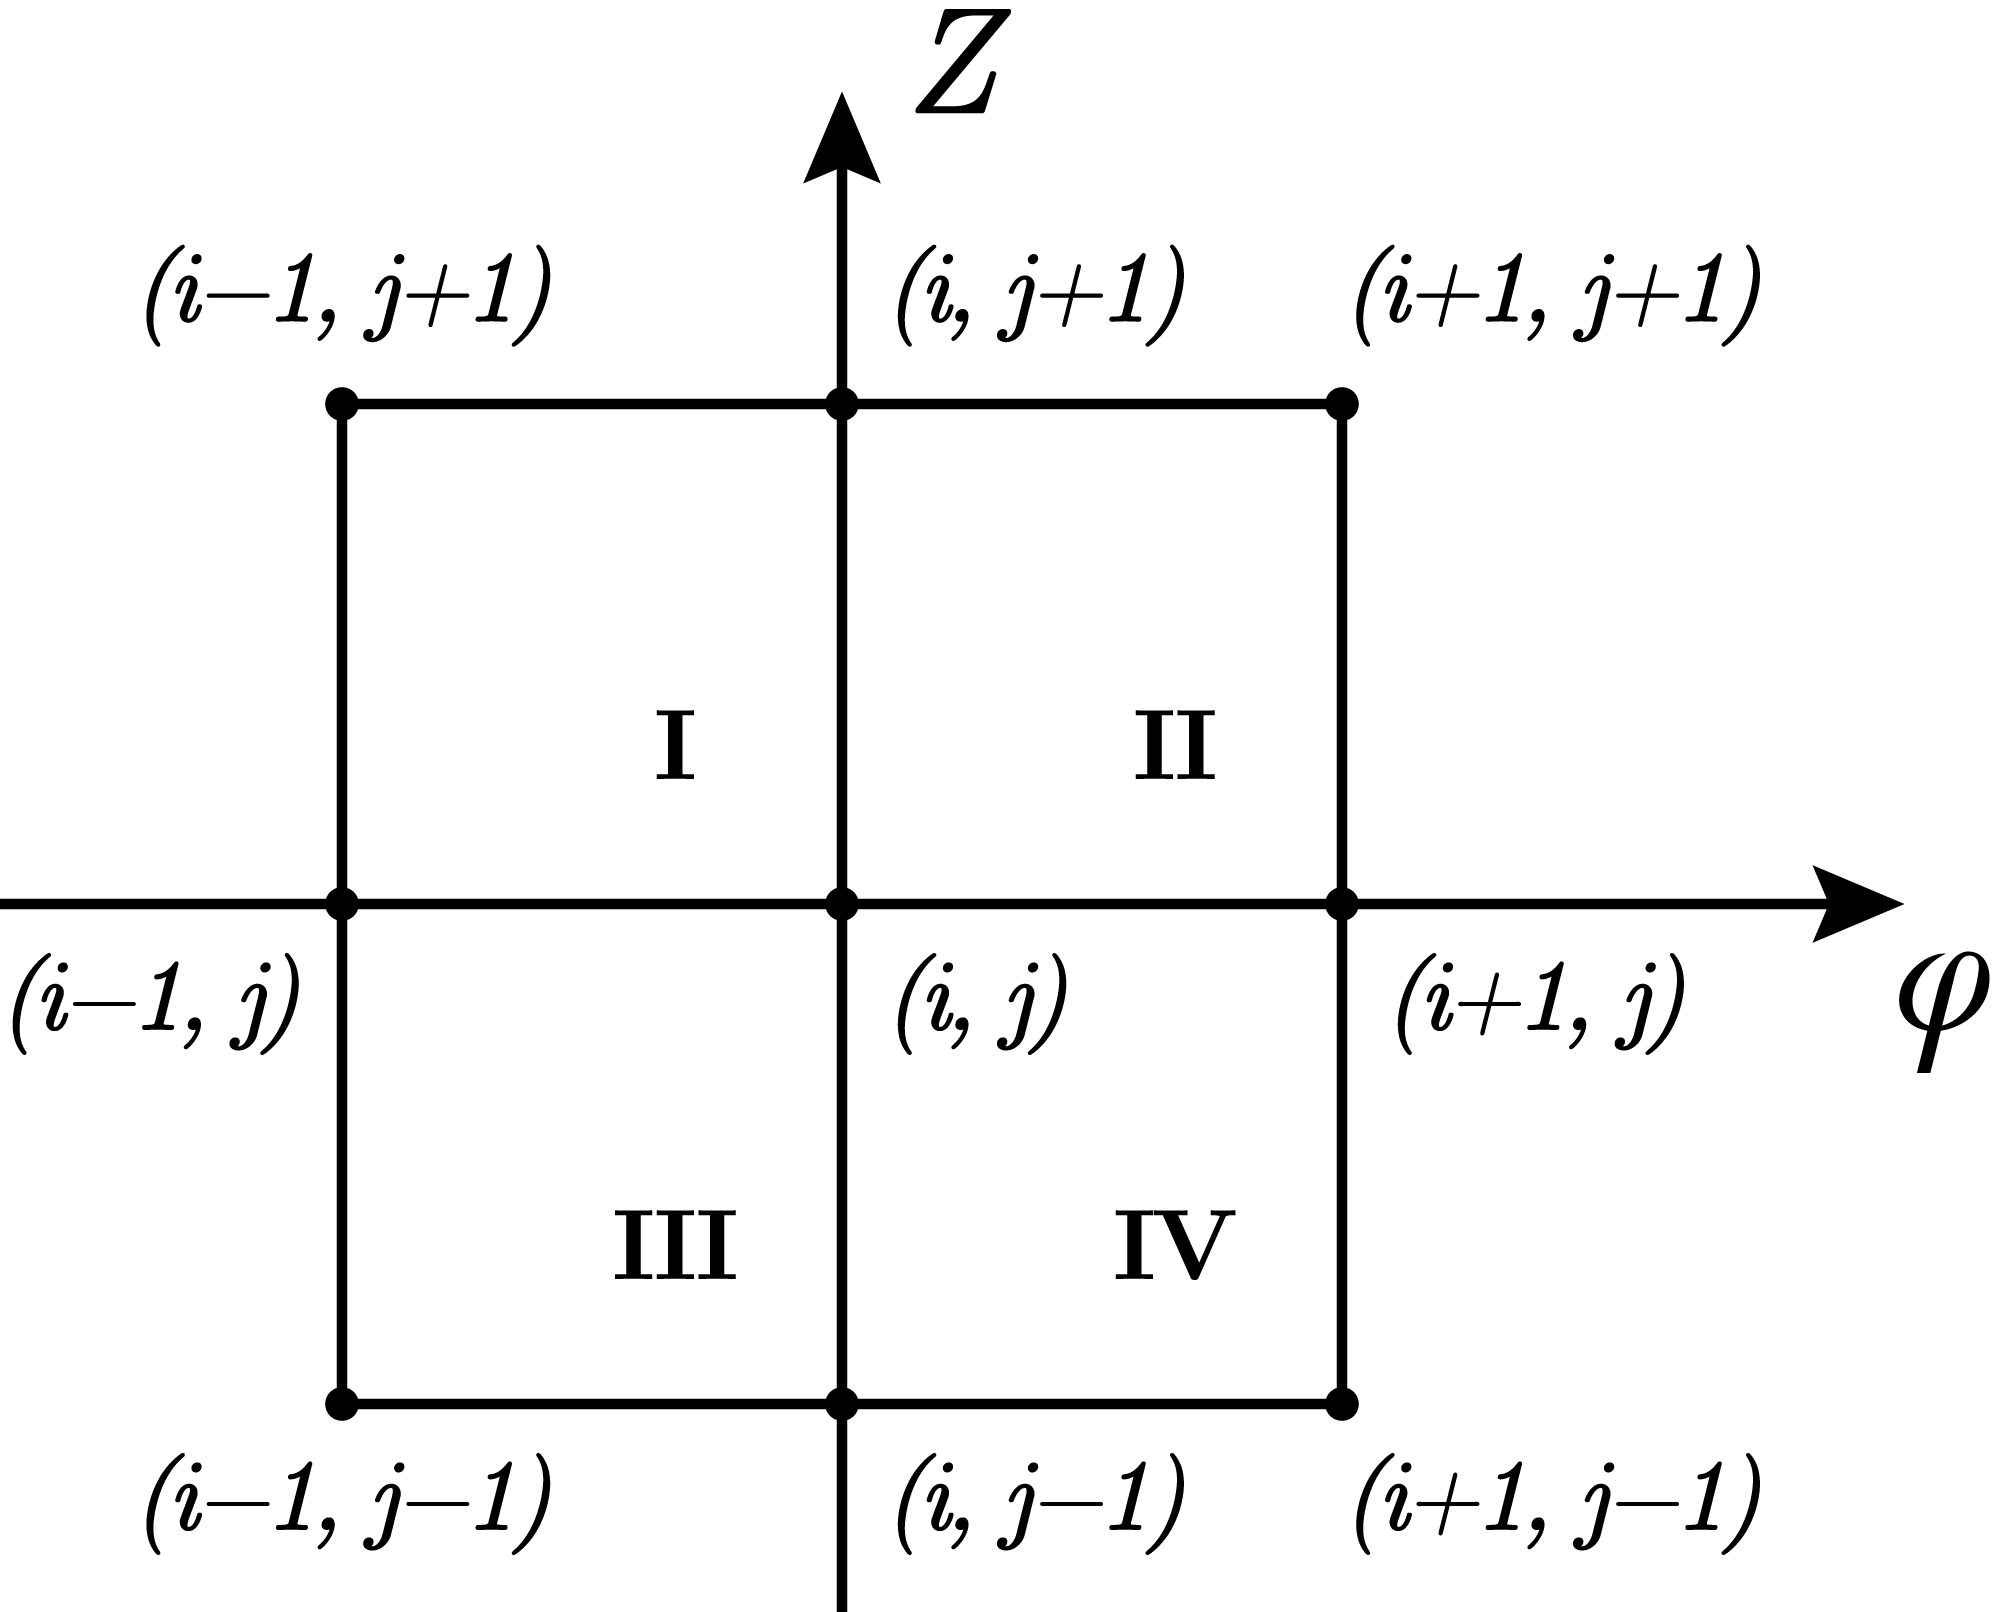
\includegraphics[scale=0.5]{square}}

\caption{Девятиточечный шаблон, на котором реализуется разностная схема; аппроксимации (\ref{scheme_mixed}) относятся к квадратам I, II, III, IV.}
\end{figure}

Можно показать, что при постоянных эффективных коэффициентах диффузии и подходящих краевых условиях будет иметь место конечномерный аналог соотношения (\ref{integral}):
\begin{gather}
\dfrac{\partial}{\partial t} \sum_{i, j} (n_{i, j})^2 = - \sum_{i, j}\left(K_1 \dfrac{n_{i, j} - n_{i-1, j}}{\Delta z} + K_2\dfrac{(n_{i, j} - n_{i, j-1})^2}{a \Delta \varphi}\right)^2 -\nonumber \\  - \sum_{i, j}\left(K_1 \dfrac{n_{i+1, j} - n_{i, j}}{\Delta z} + K_2\dfrac{(n_{i, j+1} - n_{i, j})^2}{a \Delta \varphi}\right)^2.
\label{integral_discrete}
\end{gather}
В случае постоянных коэффициентов для такого рода схем можно показать абсолютную устойчивость при положительной определенности их матрицы [9]. 

Рассмотренный выше метод применен и для аппроксимации производной $\dfrac{\partial n}{\partial\varphi}$ в верхнем краевом условии в точке $(N+1/2, j)$, согласованной с аппроксимацией уравнения (\ref{main_eq}) во всей области. При этом в случае положительного знака $\sin I$ аппроксимация имеет вид: \begin{equation}\dfrac{1}{2}\left(\dfrac{n_{N+1, j+1}-n_{N+1, j}}{\Delta\varphi} + \dfrac{n_{N, j} - n_{N, j-1}}{\Delta\varphi}\right),\end{equation} а в случае отрицательных значений $\sin I$ используется полусумма \begin{equation}\dfrac{1}{2}\left(\dfrac{n_{N+1, j}-n_{N+1, j-1}}{\Delta\varphi} + \dfrac{n_{N, j+1} - n_{N, j}}{\Delta\varphi}\right).\end{equation}

Для аппроксимации оператора $DTr(n_i)$, описывающего процесс <<оседания>>, были использованы дивергентные схемы как первого порядка точности (направленные разности), так и второго (центральные разности). Алгоритм свертки, предложенный в работе [11], не использовался, поскольку условия <<хорошей>> аппроксимации метода свертки и схемы направленных разностей совпадают ($\dfrac{\tilde{u}h}{2D}<<1$, где $\tilde{u}$~---~масштаб скорости конвективных движений, то есть счетная вязкость много меньше физической вязкости).


\subsection{Аппроксимация по времени для двумерной задачи амбиполярной диффузии}

В настоящей работе исследованы два метода решения полученной эволюционной дифференциально-разностной задачи. Вследствие сформулированных особенностей задачи (\ref{main_eq}), в первом методе была использована неявная схема первого порядка~---~схема естественного фильтра, которая позволяет выбрать шаг по времени, согласованный с шагами по времени в задаче моделирования термосферы (2-4 мин) [12]. Для решения системы алгебраических уравнений использовался стабилизированный метод бисопряженных градиентов [13], который давал хорошую точность при умеренном числе итераций.

В качестве второго метода исследовался метод расщепления исходной системы уравнений на две подсистемы. Этот метод исследовался с планом на его применение в задаче четырехмерного усвоения данных [14]. Очевидно, что при наличии смешанных производных мы не можем расщепить исходный дифференциальный оператор по геометрическим переменным~---~в данном случае расщепление уместнее проводить для дифференциально-разностной задачи, применяя алгоритм, предложенный и исследованный в работах [14] для задач теории упругости, позволяющий решать задачи на дробных шагах с помощью одномерных прогонок.

На языке метода слабой аппроксимации использованный в работе алгоритм расщепления имел следующий вид. На первом шаге решалась задача диффузии в проекции на вертикальную ось $z$, включающая смешанные производные и члены, описывающие плазмохимические преобразования:
\begin{gather}
\dfrac{\partial n_i}{\partial t} = \dfrac{\partial}{\partial z}\bigg[D\sin^2 I \left(\dfrac{\partial n_i}{\partial z} + \left(\dfrac{1}{T_p}\dfrac{\partial T_p}{\partial z}+\dfrac{1}{H}\right)\right)- \nonumber\\- \dfrac{1}{a}D\sin I \cos I \left(\dfrac{\partial n_i}{\partial \varphi} + \dfrac{1}{T_p}\dfrac{\partial T_p}{\partial \varphi} n_i\right)\bigg] -
 \dfrac{1}{a\cos\varphi}\dfrac{\partial}{\partial\varphi}\left[D\sin I \cos I \dfrac{\partial n_i}{\partial z}\cos\varphi\right] +\nonumber\\ + [P-k_i n_i].
\end{gather}
На втором шаге решалась задача диффузии вдоль координаты магнитной широты:
\begin{gather}
\dfrac{\partial n_i}{\partial t} = \dfrac{1}{a^2\cos\varphi}\dfrac{\partial}{\partial \varphi}\left[D\cos^2 I \dfrac{\partial n_i}{\partial\varphi} \cos\varphi\right] +\nonumber\\
+ \dfrac{1}{a\cos\varphi} \dfrac{\partial}{\partial\varphi}\left[\left(\dfrac{1}{a}D\cos^2 I \dfrac{1}{T_p}\dfrac{\partial T_p}{\partial \varphi} - D\sin I \cos I \left(\dfrac{1}{T_p}\dfrac{\partial T_p}{\partial z} + \dfrac{1}{H}\right)\right)n_i \cos\varphi\right].
\end{gather}


Для уменьшения ошибки аппроксимации использовался двуциклический вариант метода расщепления [15]. Такое расщепление позволяет естественным образом расщепить краевые условия. Обе задачи решаются одномерными прогонками вдоль соответствующих направлений. При формировании прогонок на первом шаге расщепления частично использовались идеи, предложенные в работе [16] (алгоритм типа метода Зейделя при расчете значений функций в узлах, не входящих в направление прогонки).

Коротко остановимся на проблеме неотрицательности решения. Вообще говоря, матрицы, которые необходимо обращать на каждом шаге по времени, не удовлетворяют определению М-матрицы: при выбранных пространственных шагах и значениях параметров задачи нарушение происходит в малой окрестности экватора. Для случая возникновения отрицательных значений компонент решения в алгоритме предусмотрено применение простого монотонизатора.

Детальное описание результатов версии модели ионосферы в квазиодномерной постановке, соответствующей первому шагу расщепления без учёта смешанной производной и детали используемых схем приведены в [17].

\subsection{Решение уравнения переноса}

Для решения уравнения переноса использовалась схема <<кабаре>>, являющаяся схемой второго порядка по пространству и времени на гладких решениях и при решении однородного уравнения переноса. В случае использования монотонной версии этой схемы порядок аппроксимации схемы по пространству несколько понижается. Также порядок аппроксимации схемы по времени понижается до первого при использовании схемы расщепления по физическим процессам при решении неоднородного уравнения переноса. Численные эксперименты показали устойчивость и монотонность данной схемы при числах Куранта меньше 0.5.

%Схема имеет второй порядок аппроксимации по пространству на гладких монотонных профилях и первый порядок аппроксимации по времени, если  $f \neq 0$, и второй порядок аппроксимации по времени, если $f=0$.

\vspace{5mm}

Остановимся отдельно на случае, когда уравнение переноса решается как часть общего уравнения (\ref{main_eq}) с применением метода расщепления. При этом неадвективные тенденции из уравнения переноса (\ref{transf_eq}) вычисляются неявным образом с помощью решения уравнения  \begin{equation}\label{nonadv}
\dfrac{\partial \rho}{\partial t} = f.
\end{equation}
Тогда, зная $\rho_{i, j, k}^n$ и $\overline{\rho}_{i, j, k}^{n+1}$~---~значения сеточной функции до и после решения уравнения (\ref{nonadv}), вычисляем сеточные значения неадвективных тенденций по формуле \begin{equation}\label{rhs_adv} f_{i, j, k}^n = \dfrac{\overline{\rho}_{i, j, k}^{n+1}-\rho_{i, j, k}^n}{\tau}. \end{equation}
После этого используем схему <<кабаре>>, вычисляя правую часть в виде (\ref{rhs_adv}) и выбирая в качестве начальных данных значение на $n$-ом шаге по времени $\rho_{i, j, k}^n$, а не $\overline{\rho}_{i, j, k}^{n+1}$, как это делается в обычном методе расщепления по времени.

Справедливость данного подхода можно установить, если сложить уравнения (\ref{predictor}) и (\ref{corrector}). При этом получим  уравнение вида \begin{equation} \dfrac{\rho_{i, j, k}^{n+1} - \rho_{i, j, k}^n}{\tau} + \mathrm{DIV}_{i, j, k}^{n+1/2} = f_{i, j, k}^n,\end{equation} где $\mathrm{DIV}_{i, j, k}^{n+1/2}$ аппроксимирует $\nabla(\vec{u}\rho)$ в некоторой точке сетки. Подставляя вычисленную правую часть (\ref{rhs_adv}), получим \begin{equation} \dfrac{\rho_{i, j, k}^{n+1} - \overline{\rho}_{i, j, k}^{n+1}}{\tau} + \mathrm{DIV}_{i, j, k}^{n+1/2} = 0,\end{equation} то есть решается уравнение переноса с нулевой правой частью и начальными данными, полученными в качестве результата после первого шага расщепления. Таким образом, предложенный алгоритм учёта правой части эквивалентен стандартному методу расщепления.

\section{Результаты численных экспериментов для двумерной задачи амбиполярной диффузии}


\subsection{Воспроизведение дневного вертикального профиля электронной концентрации}
\subsectionmark{Воспроизведение дневного вертикального профиля электронной концентрации}

Одним из первых и основных численных экспериментов является эксперимент по воспроизведению дневного стационарного распределения электронной концентрации. Фиксируется постоянное значение функции фотоионизации $P(z, t)$, затем расчет запускается с произвольных (для простоты~---~с нулевых) начальных данных. В ходе экспериментов проведено детальное исследование свойств сходимости решения разностной задачи к стационарному при фиксированном дневном значении фотоионизации $P$, рассмотрены пространственные характеристики стационарного решения разностной задачи при реализации описанных выше разностных схем. 

При проведении численных экспериментов были использованы шаг по пространству $h = 5$~км и по времени $\tau = 3$~мин, что соответствует характеристикам модели термосферы ИВМ РАН.

Эксперимент показал, что имеет место сходимость к стационарному распределению электронной концентрации. В этом распределении при фиксированной широте воспроизводится стационарный вертикальный профиль, близкий к наблюдаемому в средних широтах невозмущенному профилю F-слоя Земной ионосферы [13] с характерным временем установления порядка $4-5$ часов. При этом на любой фиксированной высоте максимальное значение концентрации достигается в экваториальной области.

\begin{figure}[H]
\center{
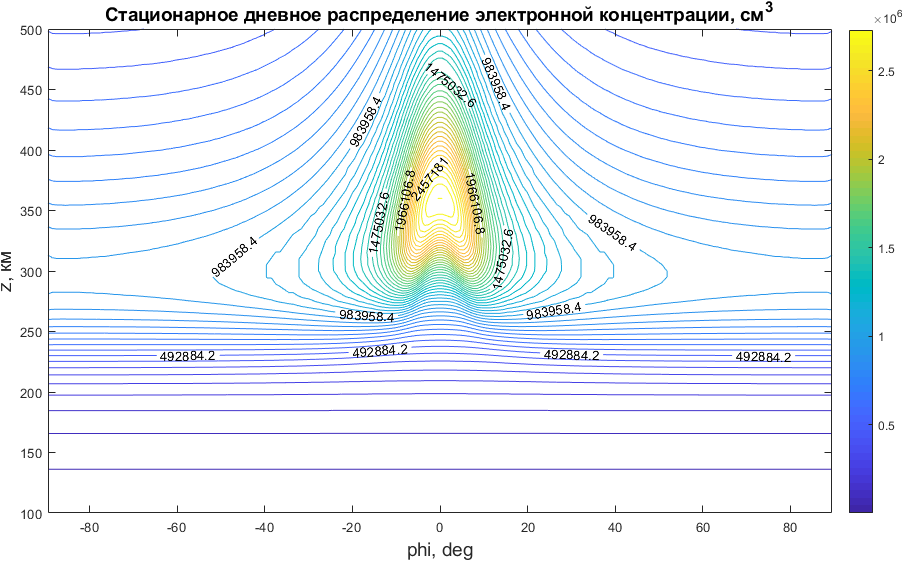
\includegraphics[scale=0.7]{2d_stationary_isoline}}

\caption{Высотно-широтное распределение электронной концентрации (см$^{-3}$) по результатам расчета стационарного дневного распределения в двумерной модели амбиполярной диффузии-плазмохимии.}
\end{figure}


\subsection{Исследование ошибки численного метода на основе аналитического решения для двух методов интегрирования по времени}

Для исследования точности используемых разностных схем рассмотрим модельное решение, на качественном уровне отражающее поведение реальной ионосферы при решении исходной задачи. Форсинг для рассматриваемой модели был рассчитан для получения данного решения. Рассмотрим случай фиксированного дневного распределения электронной концентрации в F слое, близкого к наблюдаемому в невозмущенной ионосфере. Вблизи нижней границы имеет место резкий рост содержания электронов с высотой до максимума F слоя, выше него наблюдается экспоненциальное падение, связанное с преобладанием диффузии. Кроме того, в широтном направлении наблюдается примерный максимум распределения электронной концентрации в экваториальной области. С учётом указанных особенностей было выбрано модельное решение вида:
\begin{equation}
n_{mod}(z, \varphi) = Ae^{-B(z-C)}(z-C)\cos^2\dfrac{\varphi}{2},
\label{n_mod}
\end{equation}
где положительные константы $A$, $B$ и $C$ в тестовых расчетах были выбраны равными $3\cdot 10^6$~см$^{-3}\cdot$км$^{-1}$, $1/133$~км$^{-1}$ и $100$~км соответственно. После выбора модельного решения прямой подстановкой в уравнение была вычислена соответствующая функция фотоионизации $P(z, \varphi)$ и соответствующий поток $Fz(\varphi)$ в верхнем граничном условии.

Численные эксперименты по сходимости к стационарному решению показали высокую точность результатов расчета с помощью обоих используемых нами методов. На рисунке 2 приведены вид пространственного распределения заданного аналитического решения и распределение ошибок по результатам численных экспериментов на сетке с шагом $h = 5$~км по высоте и шагом $\Delta\varphi = 1^\circ$ по широте. Видно, что максимальная численная ошибка обоих методов наблюдается в области приэкваториальных широт в верхних слоях ионосферы, а также в области полюсов, структуры распределения ошибки близки для обоих методов.

\begin{figure}[H]
\center{
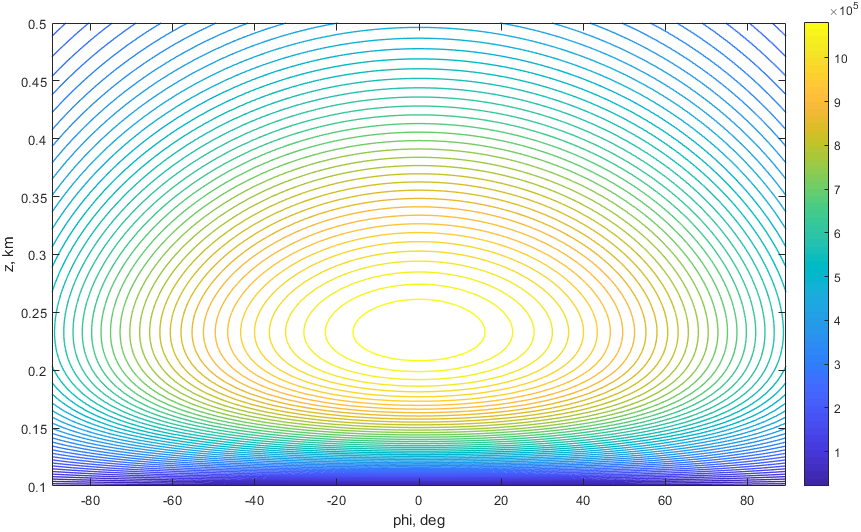
\includegraphics[scale=0.7]{model}}

(а) 

\end{figure}

\begin{figure}[H]
\center{
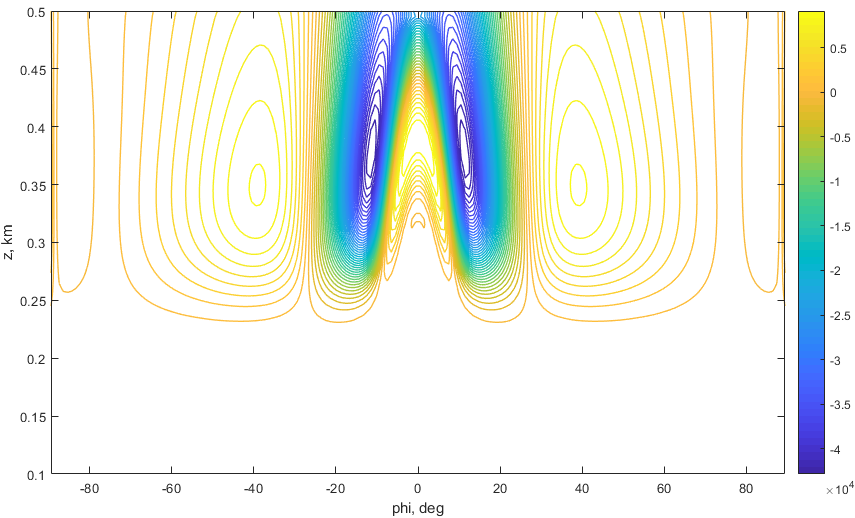
\includegraphics[scale=0.7]{error_splitted_10sec}}

(б)

\center{
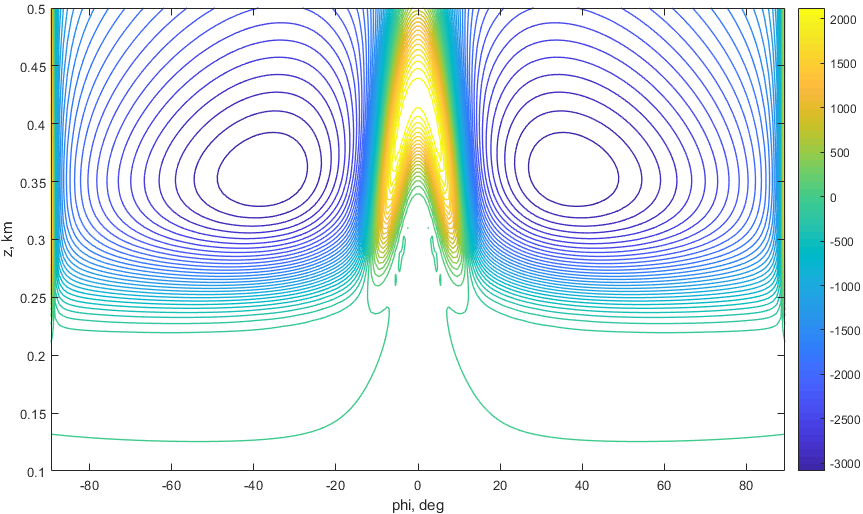
\includegraphics[scale=0.7]{error_implicit}}

(в)

\caption{Пространственный вид широтно-высотного распределения модельного аналитического решения, используемого для исследования точности (a), а также распределение ошибки при использовании расщепления и шага по времени $10$ секунд (б), а также с использованием полностью неявной схемы c шагом по времени $100$ секунд (в)}
\end{figure}


В следующих таблицах приведены некоторые результаты сравнительного анализа точности расчета стационарного решения при различных параметрах задачи. Для неявной схемы точность регулировалась выбором порядка невязки и числа итераций, шаг по времени при этом брался равным $100$~с (точность стационарного решения не зависит от него для данного метода). Точность решения методом расщепления регулируется выбором шага по времени. Расчет проводился с произвольных начальных условий на $2$ суток.

\smallskip

\begin{tabular}{|c|c|}
\hline
Относительная ошибка (C-норма)&Итерационный метод (число итераций)\\
\hline
$1\%$& 2\\
\hline
$7{,}5\%$& 1\\
\hline
\end{tabular}



\begin{tabular}{|c|c|}
\hline
Относительная ошибка (C-норма)&Расщепление (шаг по времени, с)\\
\hline
$1\%$&1\\
\hline
$7{,}5\%$&18\\
\hline
$10\%$&30\\
\hline
$15\%$&60\\
\hline
\end{tabular}

\smallskip

Итерационный метод показал более высокую точность для данной постановки задачи, при этом высокая точность достигается при использовании нескольких итераций. Для метода расщепления ошибка аппроксимации при сравнимых шагах по времени больше, для достижения той же точности, что и в неявной схеме, необходимо выбирать шаг по времени порядка $1$ с. При этом точность в $10\%$, которая считается приемлемой в задачах моделирования F слоя [1], достигается при шагах по времени порядка $30$ сек. Использование двуцикличного метода при расщеплении позволяет уменьшить ошибки на $20-30\%$.

Отметим также, что для случая неявной схемы единственное ограничение сверху на шаг по времени даёт требование сходимости итерационного процесса решения СЛАУ. Увеличение шага по времени не всегда повышает эффективность метода, поскольку это увеличивает также и требуемое количество итераций при решении линейных систем.


\subsection{Чувствительность модельного решения к потоку на верхней границе}
Для изучения роли верхнего краевого условия и получения количественных оценок проведены отдельные численные эксперименты при постановке модели с реалистичной правой частью. Используя числовые оценки параметров модели вблизи верхней границы [17], можно показать что влияние потока на верхней границе на формирование профиля электронной концентрации определяется соотношением слагаемых $\dfrac{\partial n_i}{\partial z}$, $\dfrac{1}{H}n_i$, $\dfrac{Fz(\varphi)}{D\sin^2 I}$. Таким образом, отрицательный градиент вертикального профиля концентрации определяется заданным характерным масштабом диффузионного <<оседания>>, а абсолютное значение на верхней границе определяется величиной потока.

В данной работе чувствительность к его возмущениям рассматривалась с базовым значением потока, использованным в известным моделях ионосферы  $Fz(\varphi) = \pm 10^9$~см$^{-2}\cdot$сек$^{-1}$ [2]. Величина потока $Fz(\varphi)$ варьировалась в интервале этих значений, а для оценок относительной чувствительности характерные величины потока из этого диапазона возмущались на $10-20\%$. Отдельно исследовалась чувствительность величины и положения максимума концентрации в F слое, поскольку эти два параметра ионосферы являются ключевыми для прикладных радиофизических задач. На рисунке 3 представлены высотные профили электронной концентрации, а также величины и положения максимума на разных широтах по данным соответствующих численных экспериментов. Модель показывает, что зависимость поведения решения от возмущений потока на границе незначительна, экспоненциальных характер падения концентрации с высотой и его величина практически сохраняется, однако при этом изменяется значение концентраций вплоть до максимума. Относительная чувствительность максимальна для приэкваториальных широт (величина максимума F слоя на широтах $0^\circ-20^\circ$~---~меняется на $\approx 6\%$ при изменении потока на $10\%$), чувствительность положения максимума низкая при малых возмущениях, его высота меняется примерно на 50~км при изменении потока в $2$ раза. Результаты данных экспериментов для обоих методов совпадают с высокой точностью.


\begin{figure}[H]
\center{
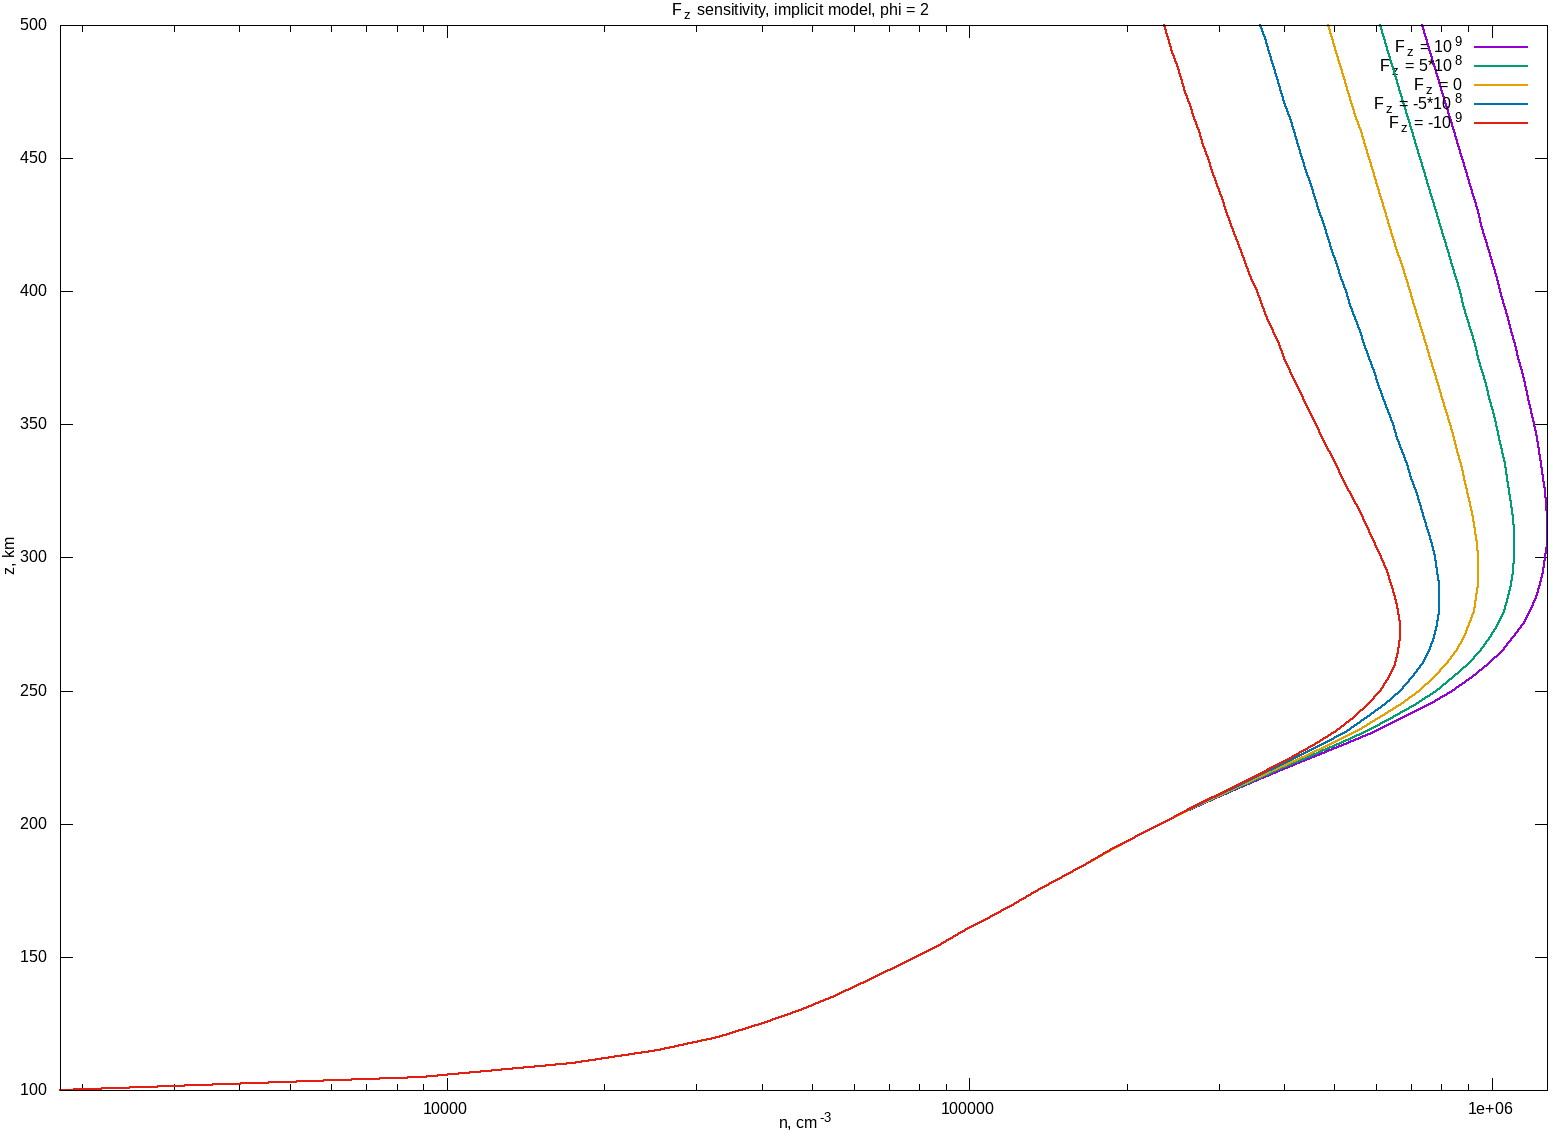
\includegraphics[scale=0.35]{sens_fz_2}}

(а) 

\end{figure}

\begin{figure}[H]
\center{
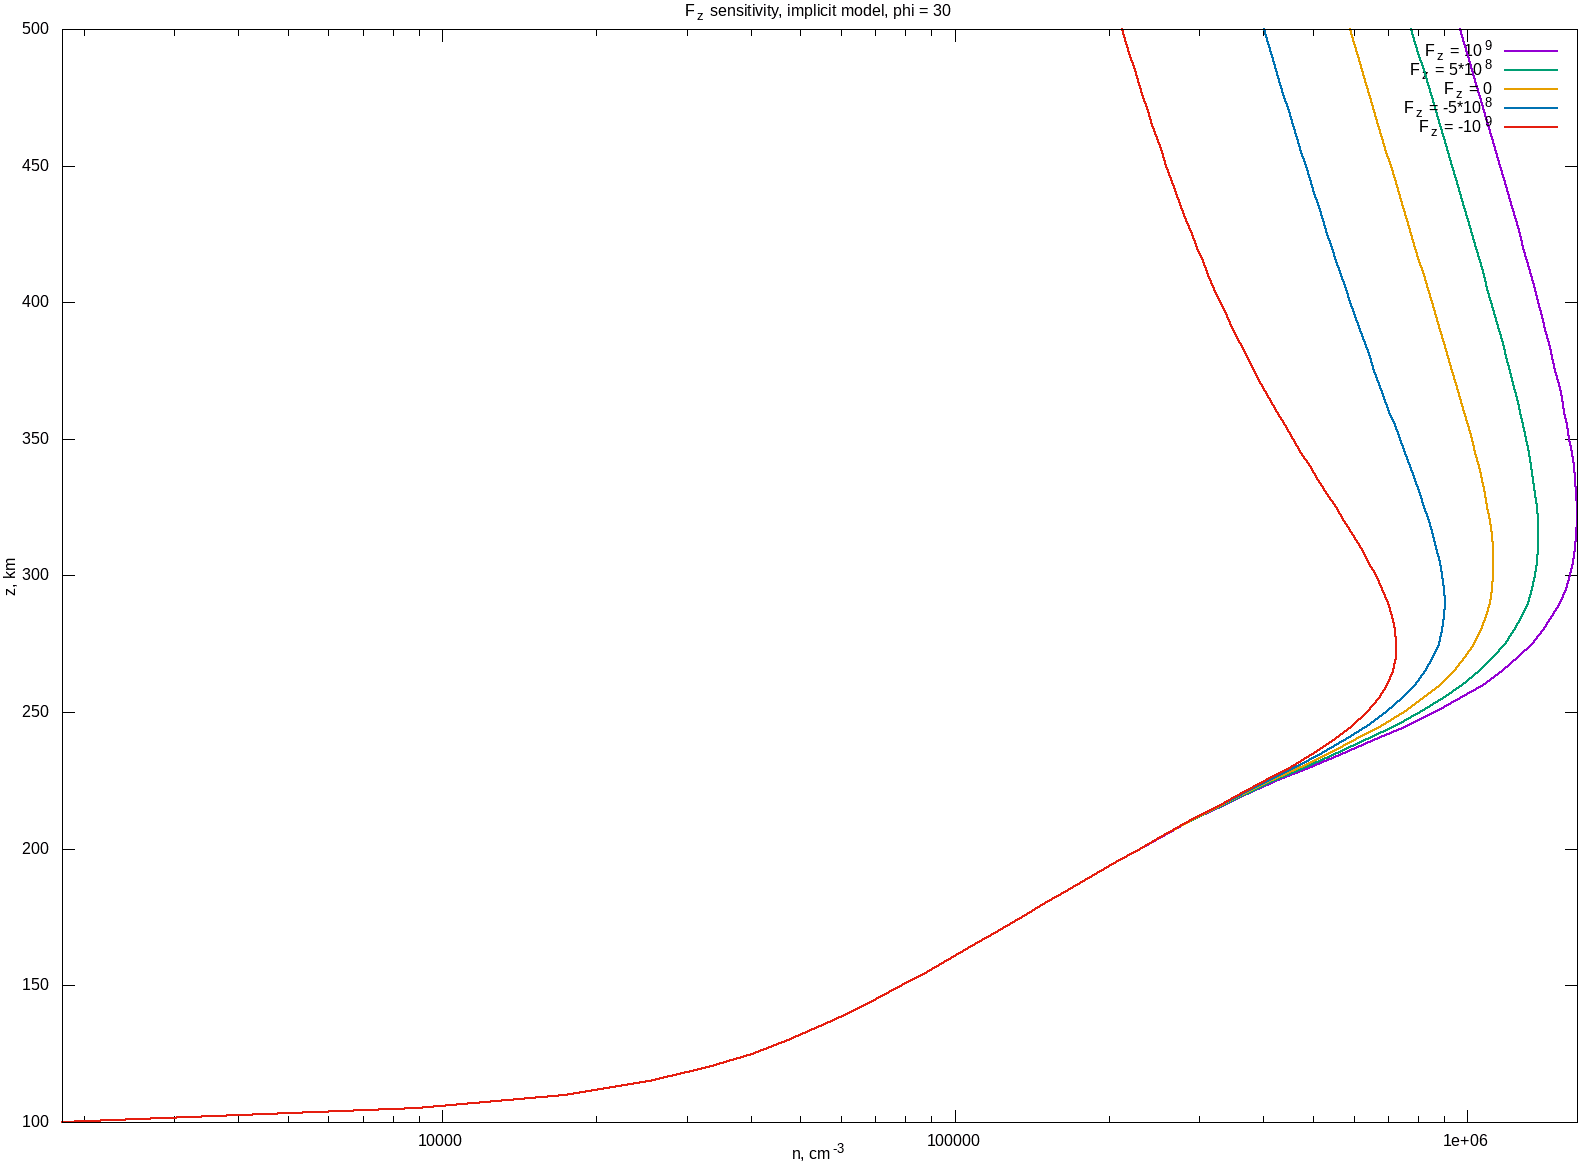
\includegraphics[scale=0.35]{sens_fz_30}}

(б)


\end{figure}

\begin{figure}[H]
\center{
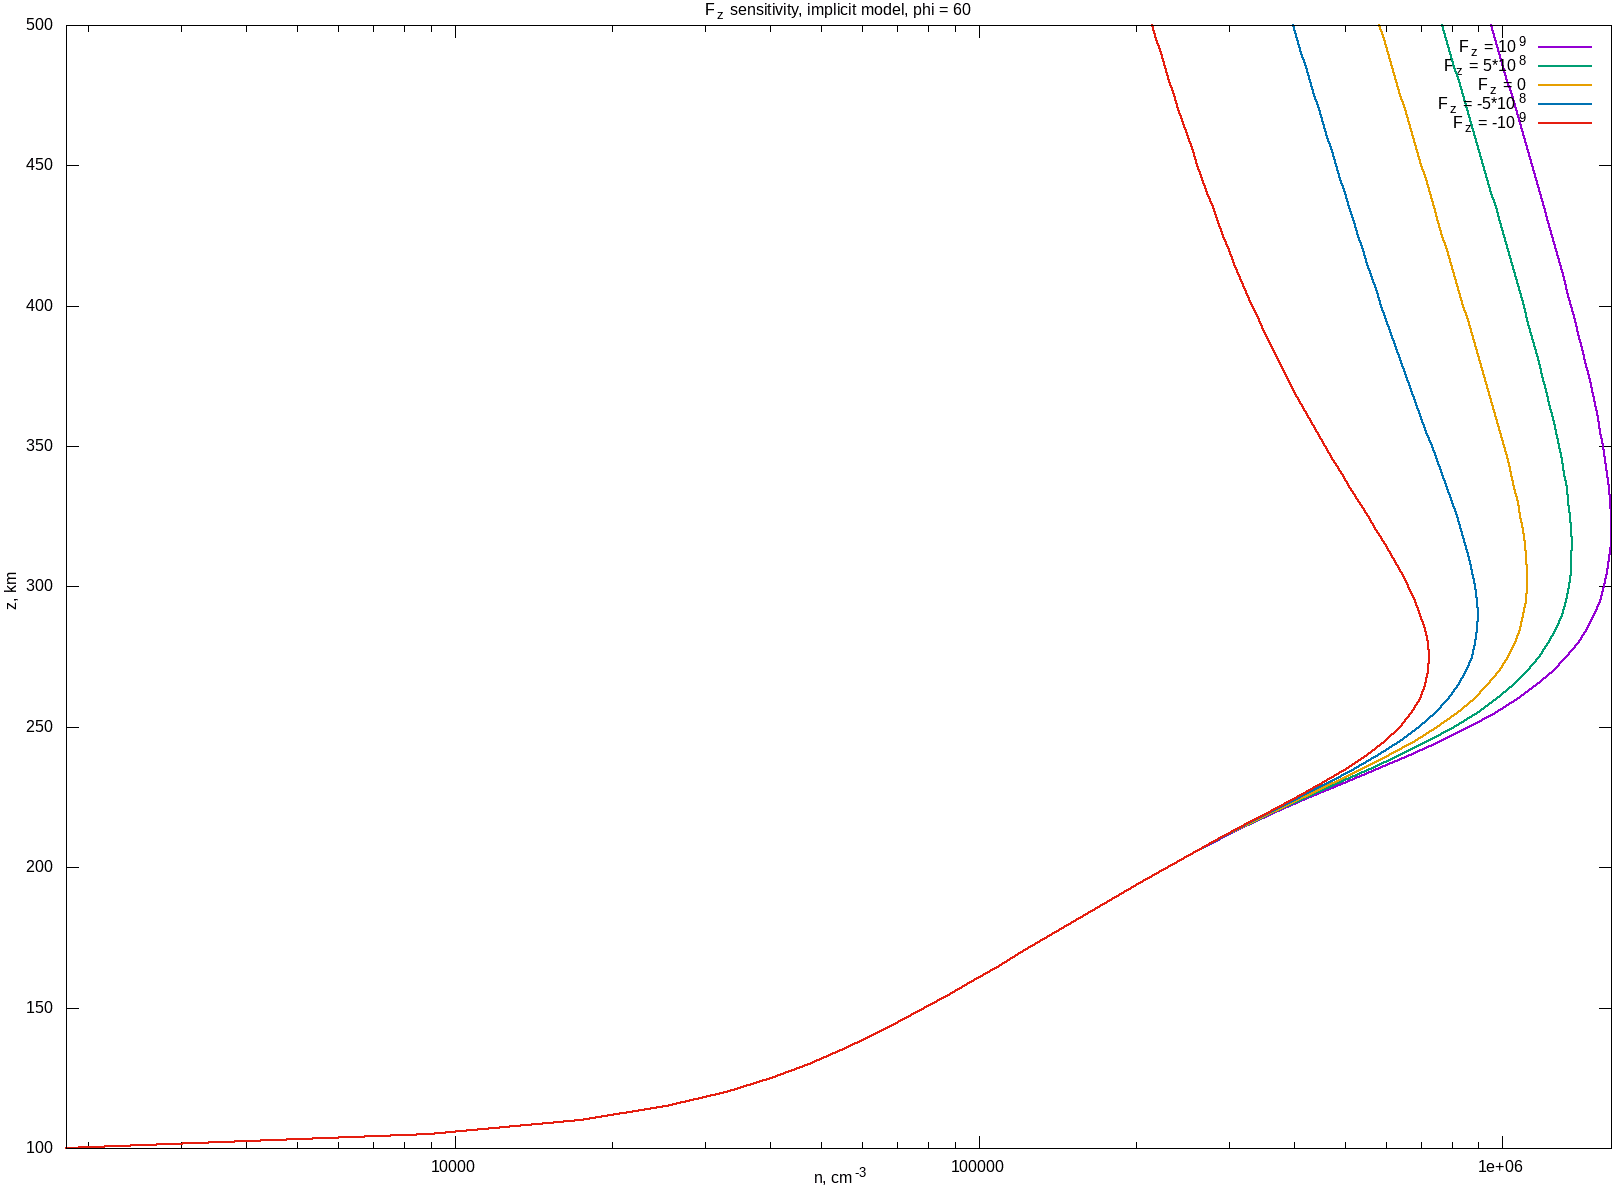
\includegraphics[scale=0.35]{sens_fz_60}}

(в)

\caption{Высотные распределения значений электронной концентрации (см$^{-3}$) при различных значениях потока на верхней границе на экваторе (а), $30^\circ$ (б) и $60^\circ$ магнитной широты по данным численных реализации модели ионосферы итерационным методом. Пространственное разрешение модели в обоих случаях составляло $5$ км по высоте, $1^\circ$ по широте, шаг по времени $10$ секунд.}
\end{figure}


%\subsection{Чувствительности ко внешним параметрам уравнения}
%\subsectionmark{Чувствительности ко внешним параметрам уравнения}







\subsection{Моделирование суточного хода}
\subsectionmark{Моделирование суточного хода}

Следующим экспериментом выступает моделирование суточного хода в соответствии с эволюцией фотоионизации с изменением зенитного угла Солнца. В ходе моделирования счет начинается с дневного значения функции $P$, а в качестве начальных значений выступает найденное дневное стационарное распределение. Затем функция фотоионизации изменяется в ходе шагов по времени. При этом результаты расчетов по обеим моделям оказываются близки, а дневное распределение спустя сутки восстанавливается в случае обоих способов интегрирования по времени: с использованием расщепления и с применением полностью неявной схемы.

На рисунках ниже приведены результаты расчетов с применением неявной схемы с шагом по времени $\tau = 100$~с на трёх фиксированных широтах: $60^\circ$, $30^\circ$ и $0^\circ$.


\begin{figure}[H]
\center{
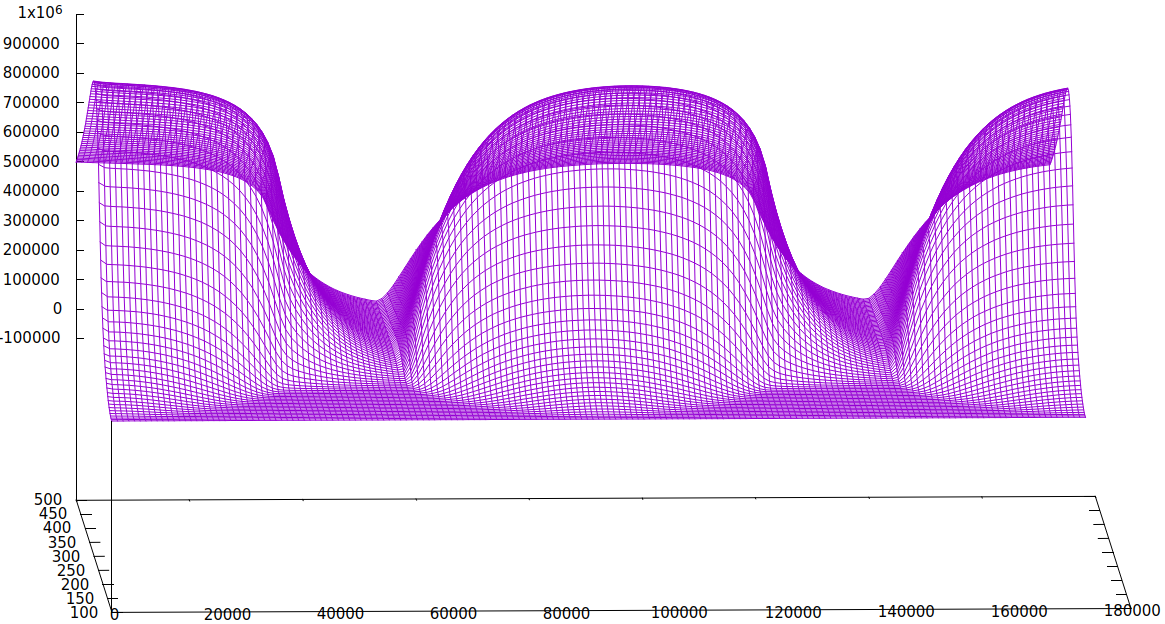
\includegraphics[scale=0.5]{implicit_2days_60}}

(а) 

\end{figure}

\begin{figure}[H]
\center{
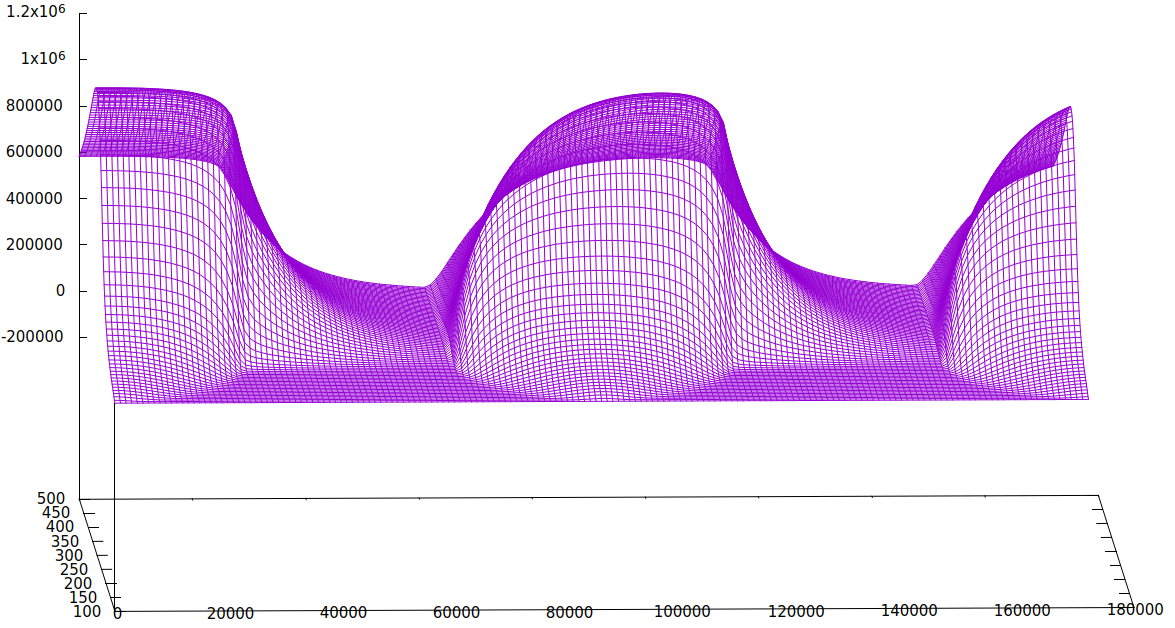
\includegraphics[scale=0.5]{implicit_2days_30}}

(б)

\end{figure}

\begin{figure}[H]
\center{
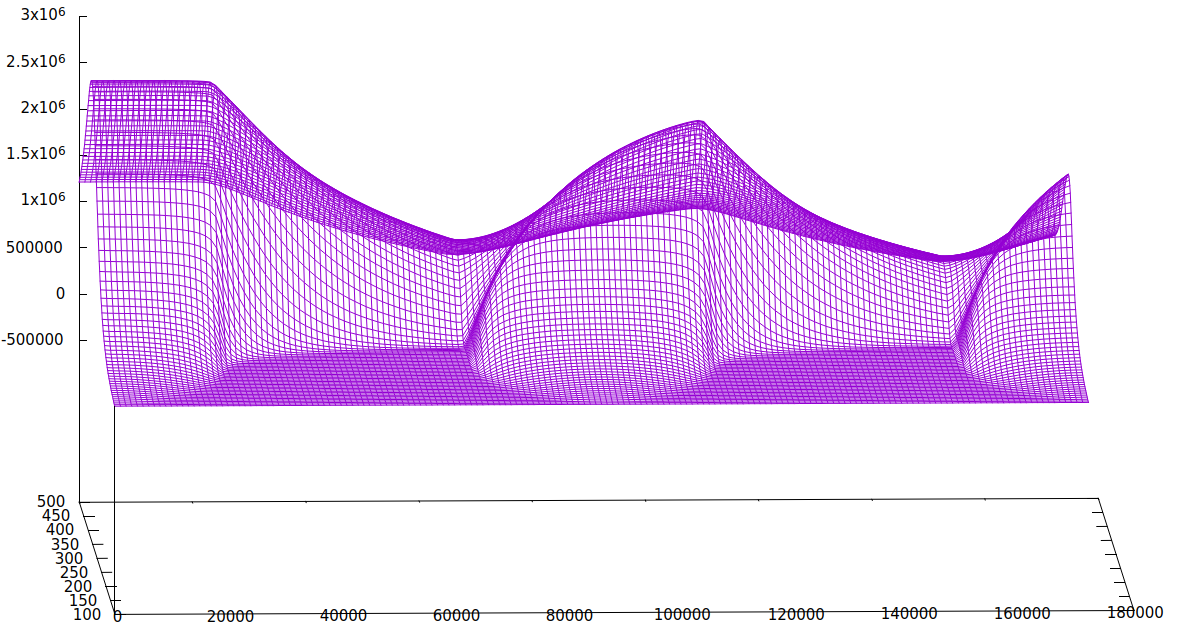
\includegraphics[scale=0.5]{implicit_2days_0}}

(в)

\caption{Результаты экспериментов по моделированию суточного хода при фиксированных широтах: $\varphi = 60^\circ$ (а), $\varphi = 30^\circ$ (б), $\varphi = 0^\circ$ (в); по горизонтальной оси отложено время в секундах, по вертикальной~---~электронная концентрация в см$^{-3}$, третье направление соответствует возрастанию высоты $z$ в км от $100$ км до $500$ км; расчет проведен на два дня.}
\end{figure}


\section{Результаты численных экспериментов для трёхмерной задачи адвекции-диффузии}

В рамках описанной в разделе 3 схемы реализации переноса и представленной схемы решения диффузионной модели ионосферы построена совместная трехмерная динамическая модель F слоя ионосферы, реализующая решение уравнения (\ref{main_eq}).

При численной реализации расщепление было организовано таким образом, что этап решения диффузионной задачи использован в качестве правой части уравнения (\ref{predictor}) при реализации схемы <<кабаре>>.

Отметим также, что расщепление верхнего граничного условия и его согласование с расщеплением оператора~---~нетривиальная задача, требующая отдельного рассмотрения. Во всех экспериментах на шаге диффузии применяется граничное условие третьего рода, соответствующее заданию потока вдоль магнитной силовой линии на верхней границе, а на шаге адвекции ставится условие Дирихле для потоковых переменных. Результаты показывают, что уменьшение шага по времени приводит к уменьшению ошибок, концентрирующихся на верхней границе расчетной области, с первым порядком.

\subsection{Тестирование численной реализации модели ионосферы на основе аналитического решения}

Для исследования точности используемого численного метода вновь рассмотрим то же модельное решение, что и в разделе 4.2:
\begin{equation}
n_{mod}(z, \varphi) = Ae^{-B(z-C)}(z-C)\cos^2\dfrac{\varphi}{2},
\end{equation}
где положительные константы $A$, $B$ и $C$ в тестовых расчетах были выбраны теми же, что и в разделе 4.2. 

Важная особенность тестирования аналитического решения состоит в необходимости расщепления не только оператора, но и форсинга в задаче: слагаемые правой части, относящиеся к диффузионной задаче, учитываются на шаге диффузии, а члены, уравновешивающие перенос, включены в соответствующий форсинг на шаге адвекции. Объединение правых частей в одну функцию с заданием только на одном из шагов расщепления (к примеру, на шаге амбиполярной диффузии) приводит к существенным ошибкам модели. В случае включения в рассмотрение нейтрального ветра скорости переноса также задаются по аналитическим формулам. Для исследования возникающей ошибки численного метода и изучения возможных особенностей в поведении ошибки рассмотрено несколько полей скорости. 

Для некоторых из использованных полей скорости проводились эксперименты с изменением амплитуды скорости (за счет изменения множителя перед соответствующими компонентами при сохранении вида самого поля). При этом для выполнения неравенства $c < 1/2$ для числа Куранта, обеспечивающего монотонность используемой модификации схемы <<кабаре>>, при решении уравнения переноса делался один шаг диффузии и несколько шагов адвекции. Во многих экспериментах скорости оказывались существенно завышенными по сравнению с реальными, но даже несмотря на это ошибка численного метода была относительно малой и сравнимой с ошибкой пространственной аппроксимации в задаче амбиполярной диффузии, рассмотренной в разделе 4.2, что подтверждает применимость использованного метода. Во всех экспериментах по пространству выбрано разрешение с шагом $h = 5$~м по высоте и шагом $\Delta \varphi = 2^\circ$ по широте.

Были проведены численные эксперименты по сходимости к стационарному решению, они показали высокую точность результатов расчета.

\subsubsection{Бездивергентное поле скорости}

В качестве одного из первых тестов было выбрано бездивергентное поле, заданное с помощью функции тока вида:
\begin{equation}\label{nondiv_field}
\psi = C_1 \cos^2 \varphi \cdot \sin \varphi \cdot \exp\left(-\dfrac{z-100}{C_2}\right)
\end{equation}
и соответствующих компонент скорости 
\begin{gather}
v_z = \dfrac{1}{a\cos\varphi} \dfrac{\partial \psi\cos\varphi}{\partial \varphi}; \ v_\varphi = -\dfrac{\partial \psi}{\partial z}.
\end{gather}
Константа $C_2$ полагалась равной $800$~км, а $C_1$ задавалась таким образом, чтобы максимальное значение модуля вертикальной скорости составляло $1600$~м/с.

Численное моделирование показало, что имеет место сходимость к стационарному решению с первым порядком по времени, причем относительная ошибка в C-норме при шаге по времени в $30$~с не превышала $1{,}3\%$ при любых использованных полях скорости. 

Профиль распределения ошибки сохраняет некоторые характерные черты профиля скорости и суммируется с ошибкой пространственной аппроксимации. В проведенных экспериментах ошибка оказывается распределена преимущественно в средних широтах. Имеет место убывание C-нормы ошибки с первым порядком при уменьшении шага по времени. 

\begin{figure}[H]
\center{
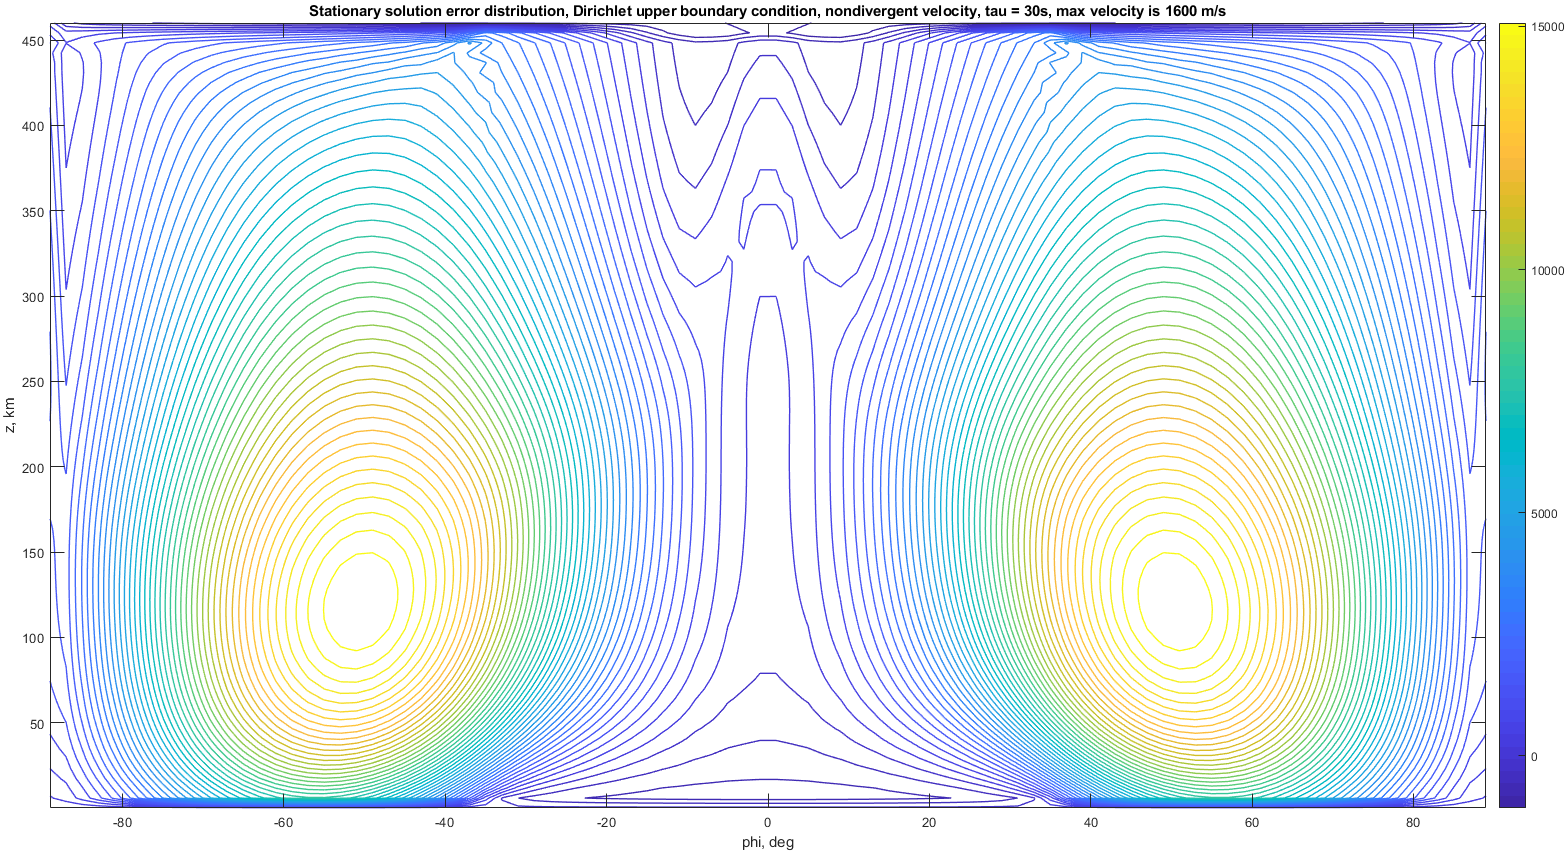
\includegraphics[scale=0.4]{nondivergent_tau_30}}

(а) 

\end{figure}

\begin{figure}[H]
\center{
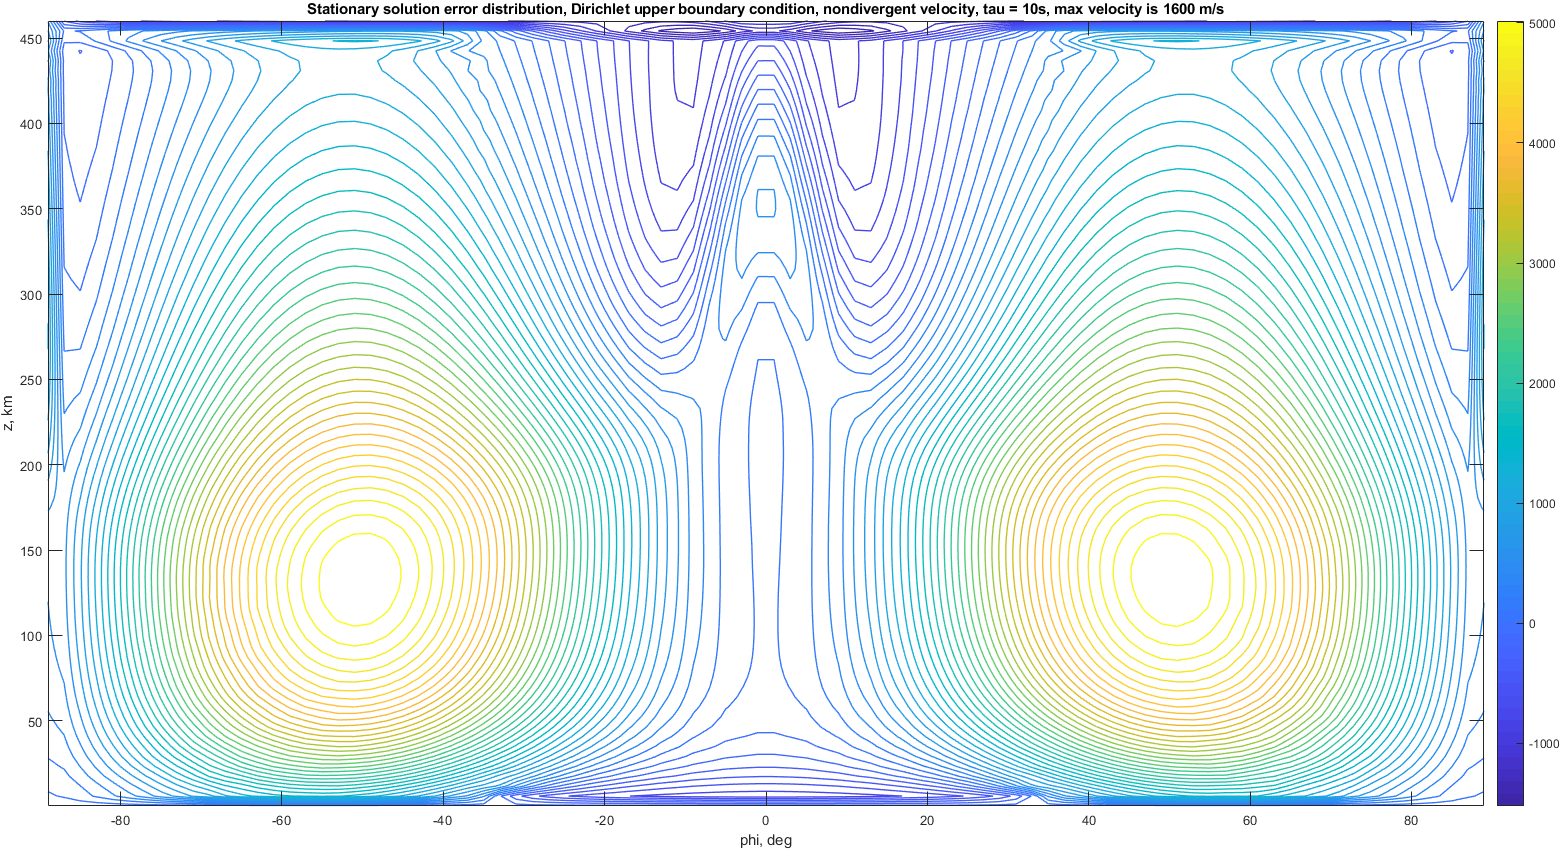
\includegraphics[scale=0.4]{nondivergent_tau_10}}

(б)

\end{figure}

\begin{figure}[H]
\center{
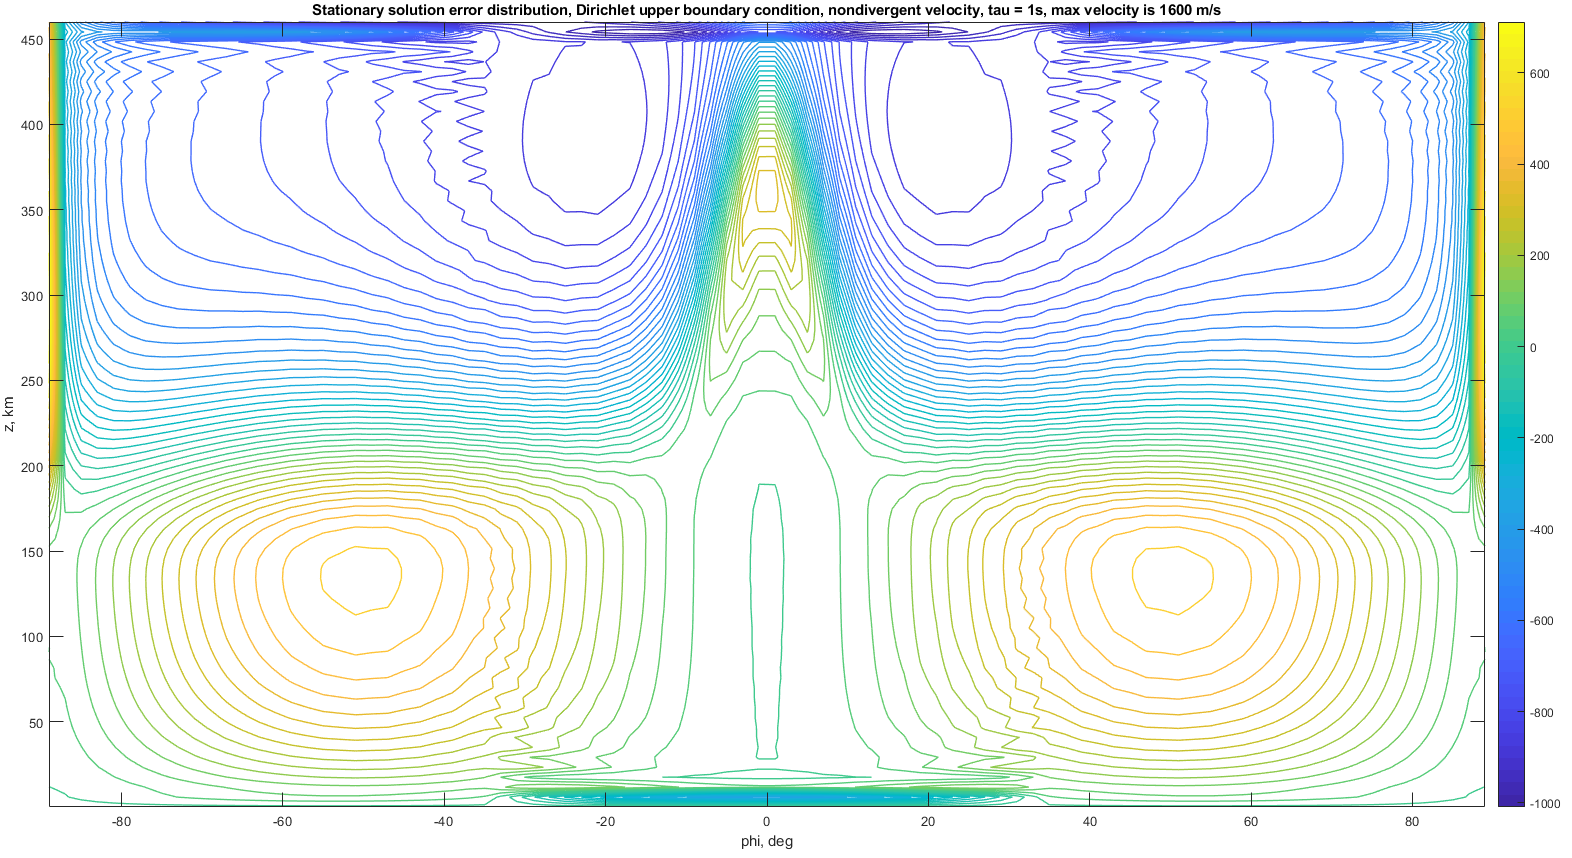
\includegraphics[scale=0.4]{nondivergent_tau_1}}

(в)

\caption{Широтно-высотные распределения ошибки численного метода при экспериментах по сходимости к стационарному решению с бездивергентным полем скорости; шаг по времени (от верхнего рисунка к нижнему) соответственно 30, 10 и 3 секунды.}
\end{figure}

Отметим, что в последнем случае основную роль играет ошибка пространственной аппроксимации, а дискретизация по времени вносит либо ошибку того же порядка, либо меньшую, дополнительная к пространственно-аппроксимационной ошибка концентрируется преимущественно ближе к верхней границе.

\subsubsection{Случай константной вертикальной скорости и влияние переноса на формирование профиля концентрации}

В качестве одного из дополнительных экспериментов была проведена проверка следующего вида: задавалось постоянное поле скорости вдоль оси $z$ величиной $200$~м/c, форсинг в уравнении задавался так, чтобы указанная выше модельная функция по-прежнему давала стационарное решение, после чего в части кода, реализующего адвекцию, скорости переноса занулялись. При этом модель сходилась к некоторому стационарному решению, вообще говоря, отличному от выбранного. Затем сравнивались полученные ошибки численного стационарного решения: со включенной и отключенной скоростью в блоке адвекции. 

\begin{figure}[H]
\center{
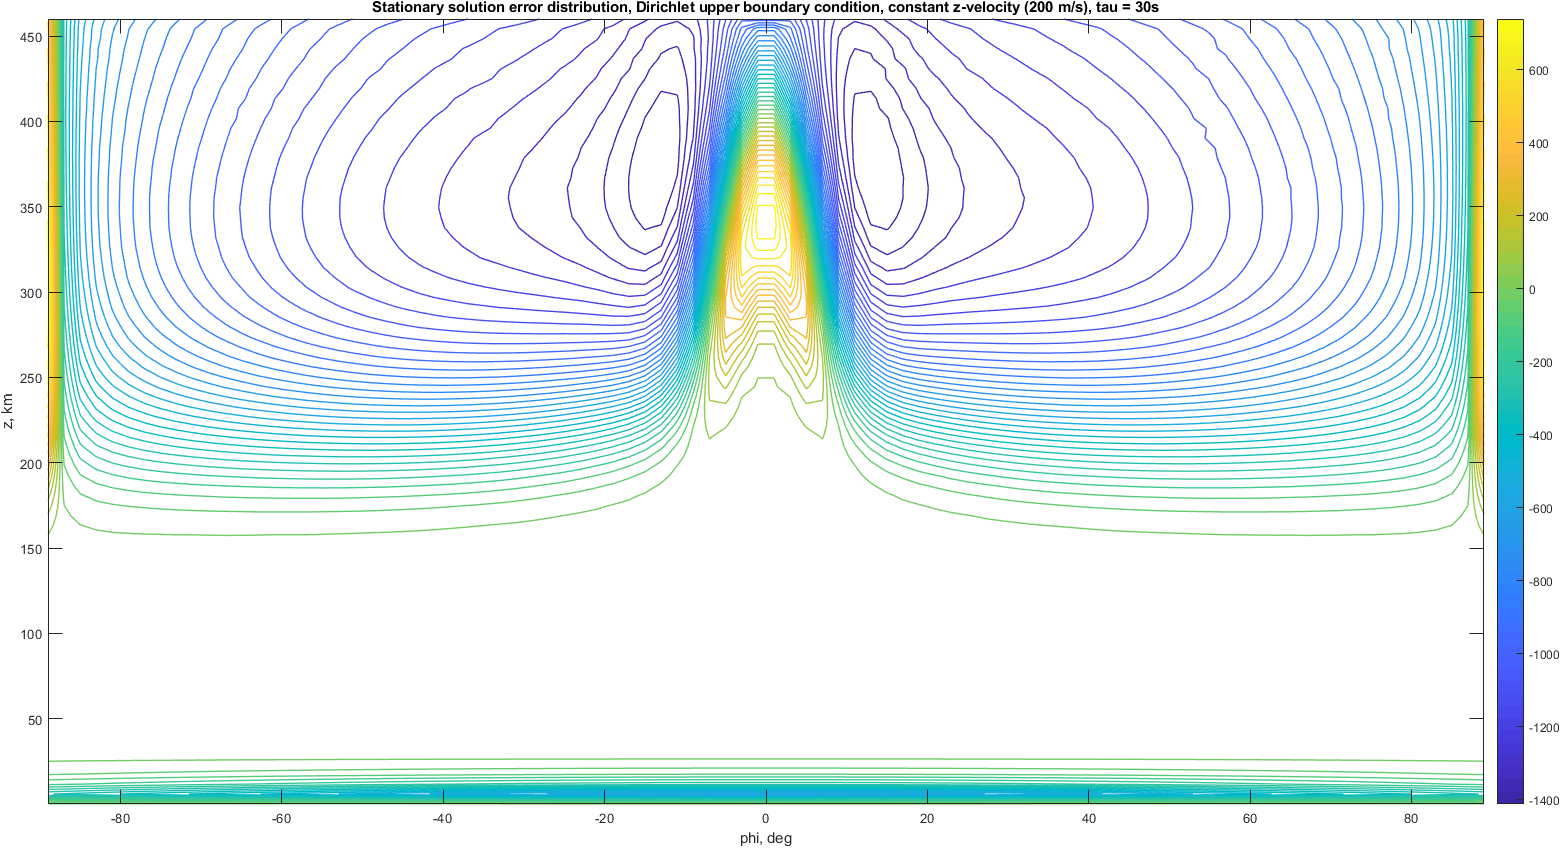
\includegraphics[scale=0.4]{const_vel_err}}

\end{figure}

\begin{figure}[H]
\center{
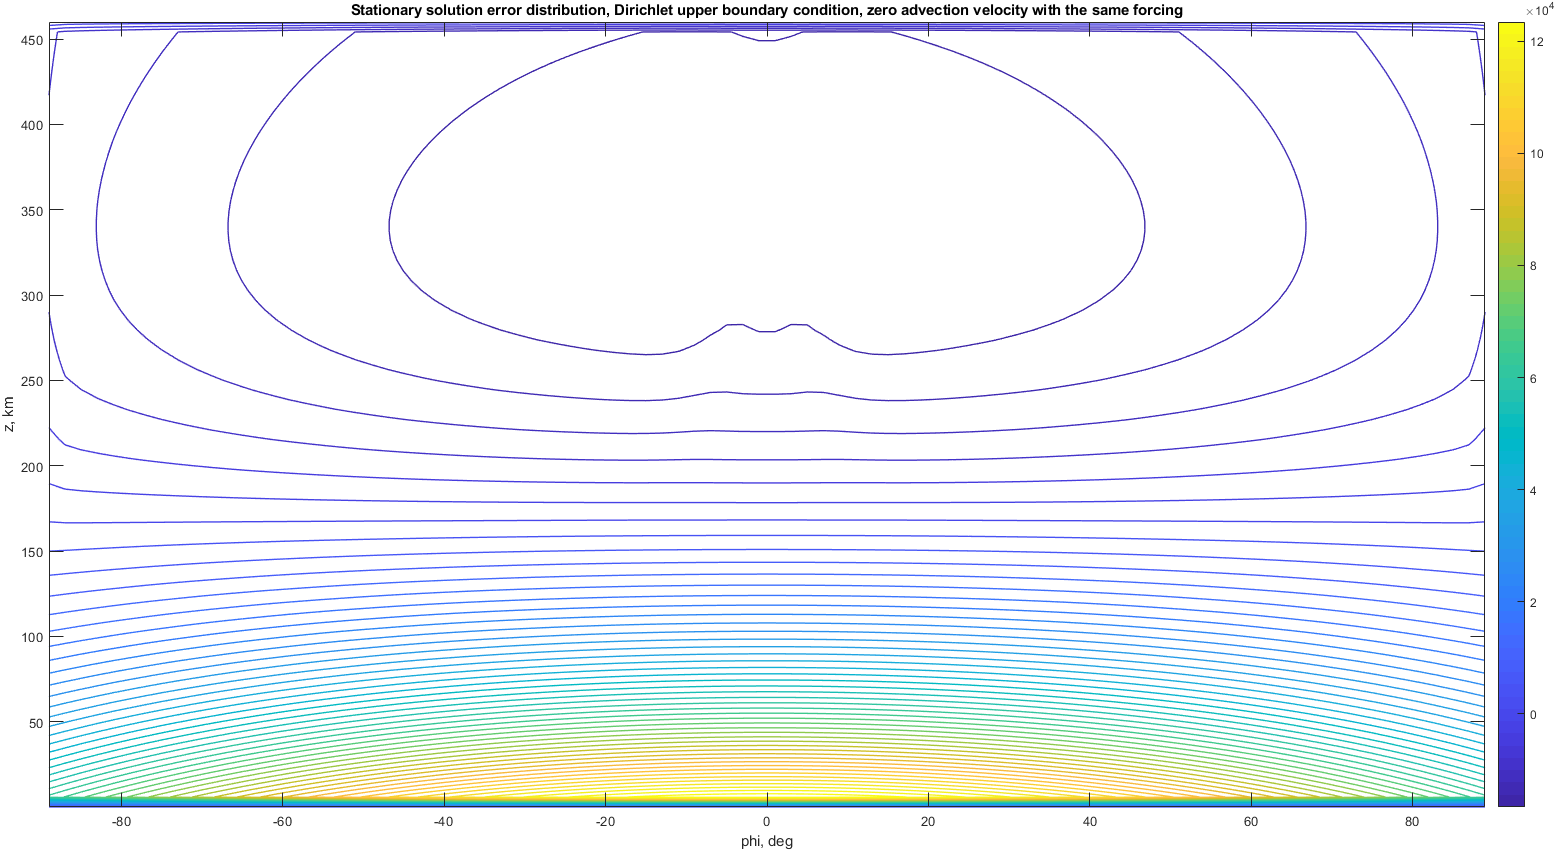
\includegraphics[scale=0.4]{const_vel_err_novel}}


\caption{Широтно-высотные распределения ошибки в эксперименте по сходимости к стационарному модельному аналитическому решению с константным вертикальным полем скорости (сверху) и с отключенным полем скорости в блоке адвекции, но тем же форсингом, что и для полной задачи (снизу)}
\end{figure}

Результаты показали существенную ошибку в вычисленном стационарном решении по сравнению с модельным решением, что означает существенный вклад переноса в рассматриваемой постановке.

\subsection{Различные дивергентные поля скорости, направленные вдоль вертикальной оси}

Помимо тестов с бездивергентным полем скорости были рассмотрены также и некоторые дивергентные поля. Ошибка численной модели изменяла характер распределения, но не преывшала уже рассмотренных выше значений. 

\subsubsection{Поле $v_z = A\cos(Bz+C)$}

В первом эксперименте задавалось вертикальное поле вида 
\begin{equation}\label{cosfield}
v_z = A\cos\left(\dfrac{z-100}{400}\pi - \dfrac{\pi}{2}\right),
\end{equation}
где $z$ задано в км, а константа $A$ выбиралась так, что максимальное по модулю значение вертикальной компоненты скорости было равно (в различных экспериментах) соответственно $1400$, $140$ и $20$~м/c соответственно. При этом ставится эксперимент как по сходимости при уменьшении шага по времени (выбираются шаги по времени $30$, $10$ и $3$ секунды при амплитуде скорости $30$~м/c), так и по исследованию зависимости ошибки от амплитуды скорости при фиксированном шаге по времени $30$ секунд. 


Результаты по исследованию сходимости при уменьшении временного шага показывают, что наибольшая ошибка при достаточно больших шагах по времени достигается вблизи верхней границы, но при уменьшении $\tau$ приходит к распределению, схожему с ошибкой пространственной аппроксимации, а при шаге по времени порядка $30$ секунд остается того же порядка. 

\begin{figure}[H]
\center{
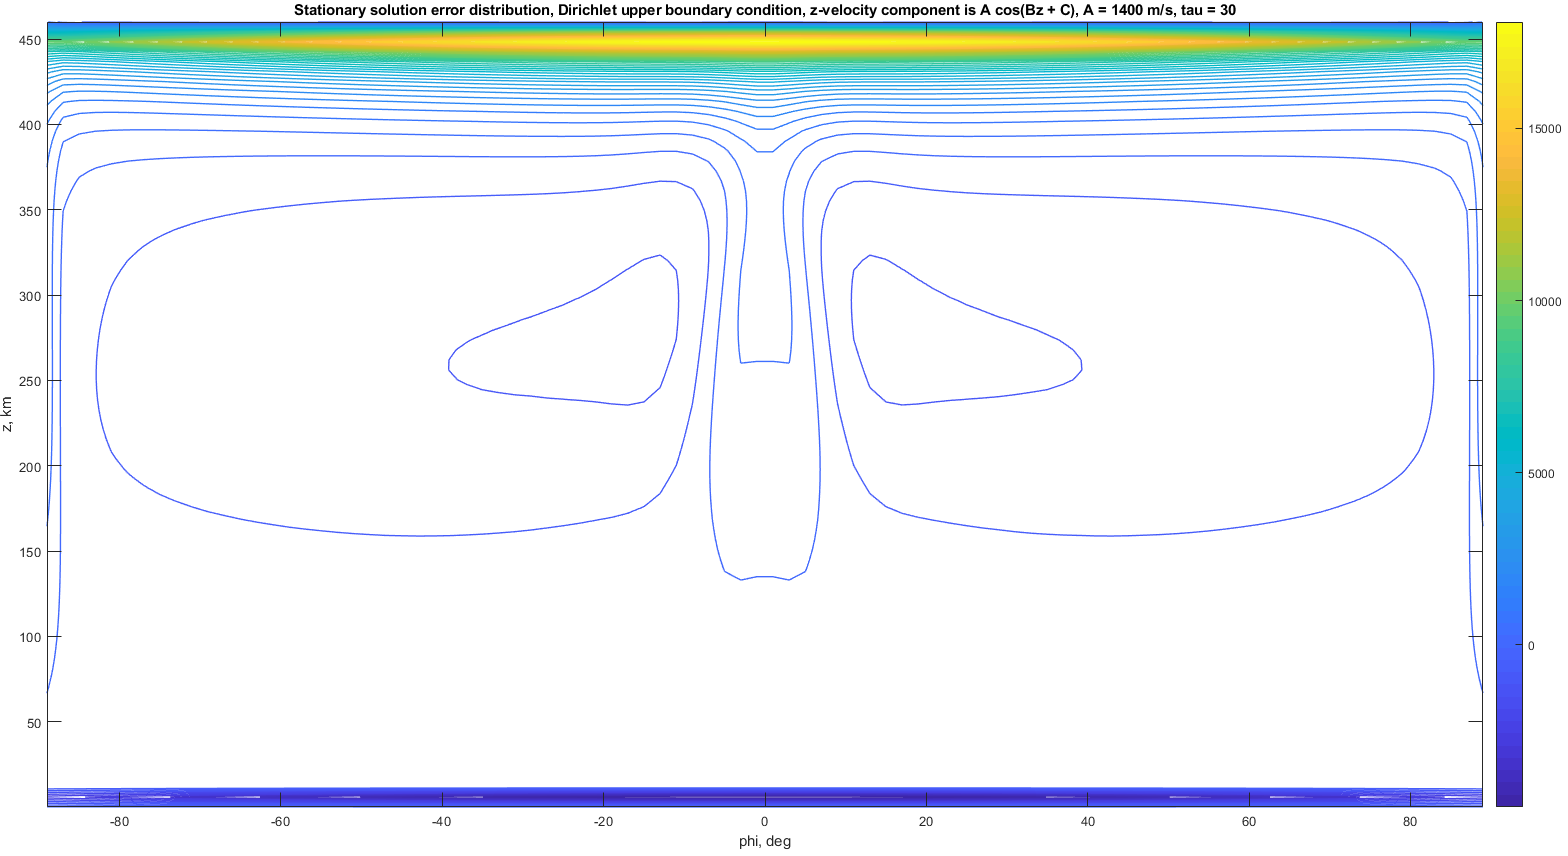
\includegraphics[scale=0.4]{cos_30sec_velocities_1400}}

(а) 

\end{figure}

\begin{figure}[H]
\center{
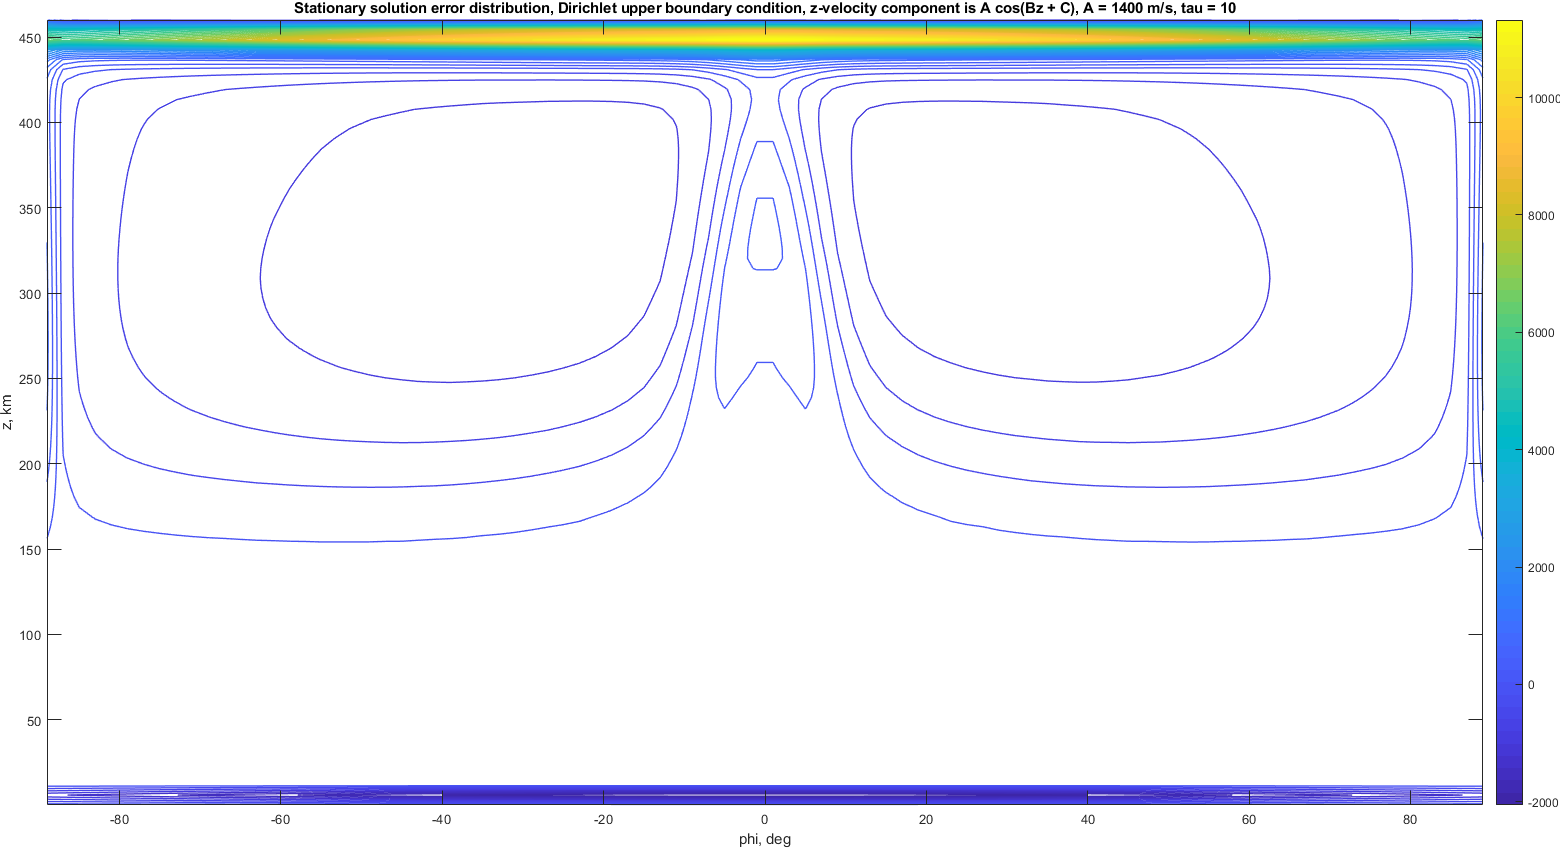
\includegraphics[scale=0.4]{cos_10sec_velocities_1400}}

(б)

\end{figure}

\begin{figure}[H]
\center{
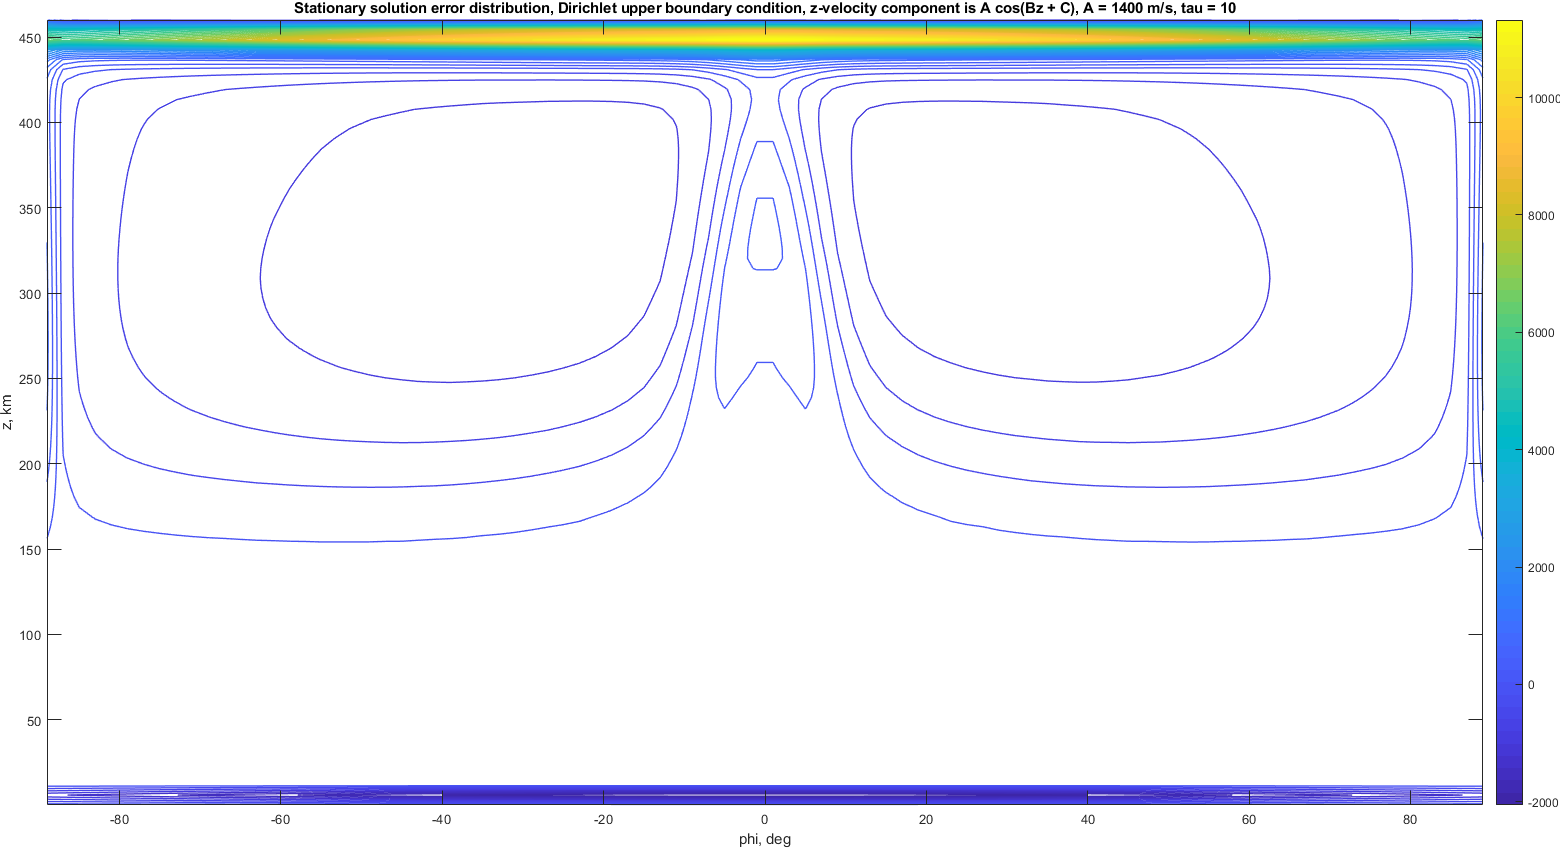
\includegraphics[scale=0.4]{cos_10sec_velocities_1400}}

(в)

\caption{Широтно-высотные распределения ошибки в эксперименте по сходимости к стационарному модельному решению с переменным вертикальным полем скорости  $v_z = A\cos(Bz+C)$; в данном эксперименте рассматривается уменьшение шага по времени, соответственно, сверху 30 c, в середине 10 с, снизу 1 с}
\end{figure}


Уменьшение амплитуды скорости с $1400$~м/с до $140$~м/с при шаге по времени $30$ секунд существенно уменьшает ошибку в случае верхнего граничного условия Дирихле.


При скоростях нейтрального ветра порядка $20$~м/c (порядка реально наблюдаемых величин) ошибка практически не меняется по сравнению с ошибкой в задаче двумерной амбиполярной диффузии. Приведем, к примеру, распределение ошибки при амплитуде $20$~м/с.

\begin{figure}[H]
\center{
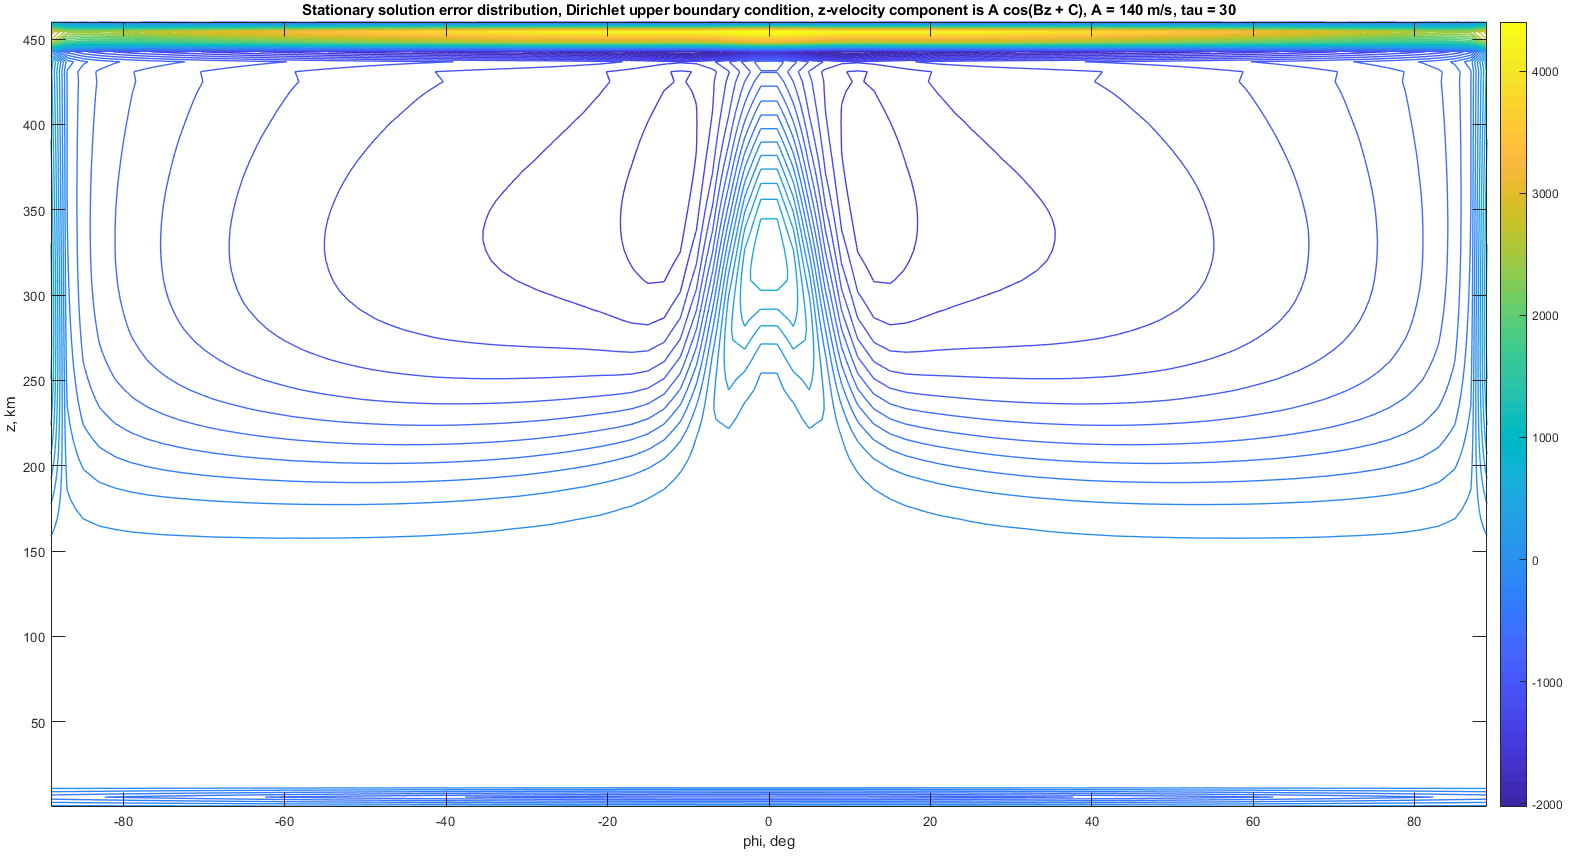
\includegraphics[scale=0.4]{cos_30sec_velocities_140}}

(б)

\end{figure}

\begin{figure}[H]
\center{
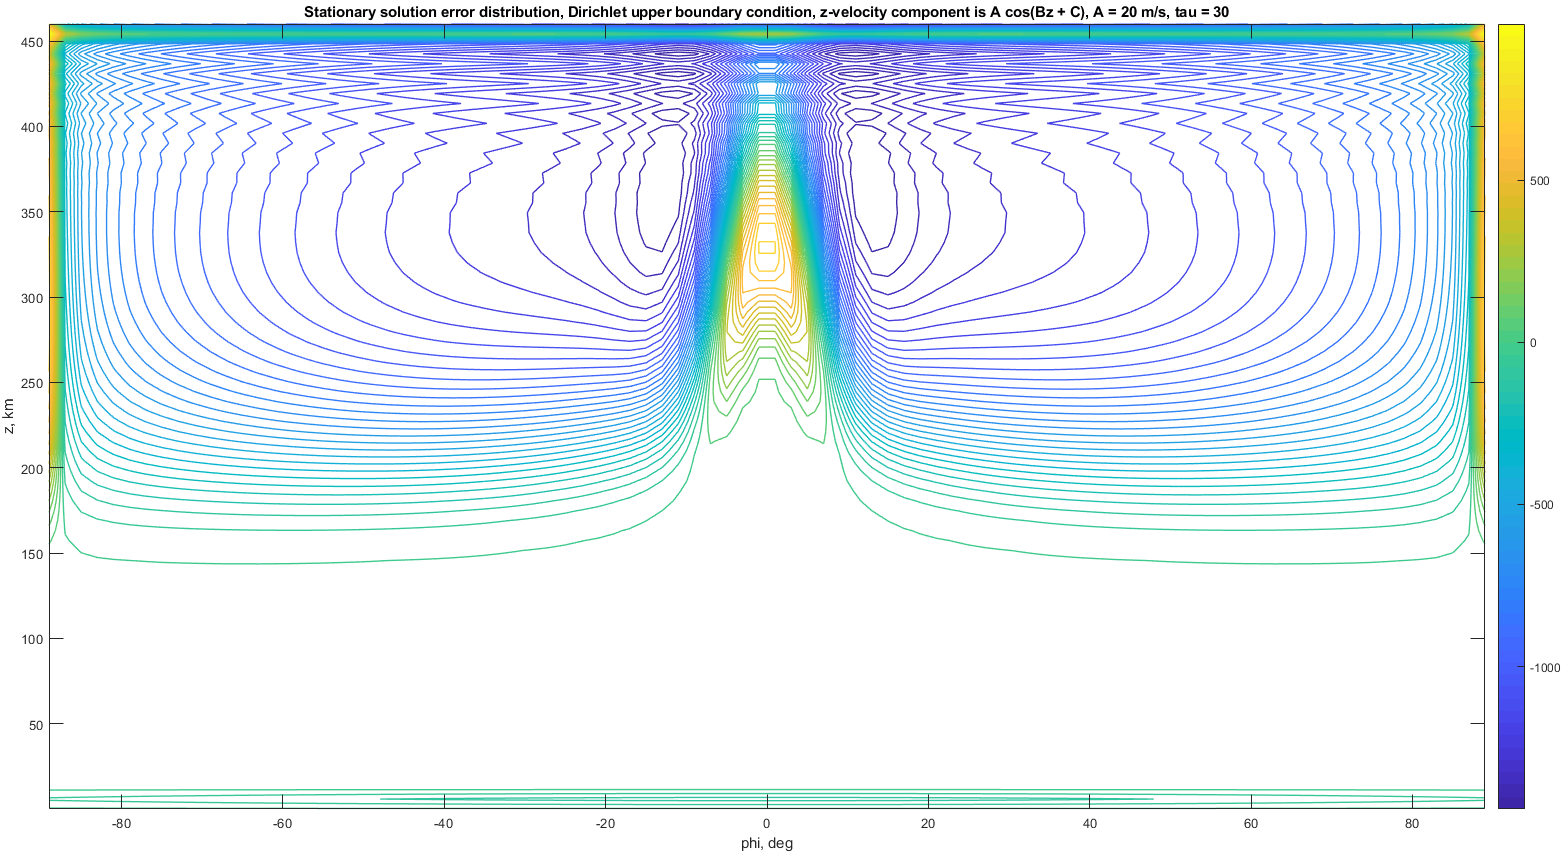
\includegraphics[scale=0.4]{cos_30sec_velocities_20}}

(в)

\caption{Широтно-высотное распределение ошибки в эксперименте по сходимости к стационарному модельному решению с переменным вертикальным полем скорости $v_z = A\cos(Bz+C)$; в данном эксперименте рассматривается уменьшенное в $10$ раз по амплитуде поле скорости, шаг по времени $30$~с (a); широтно-высотное распределение ошибки при использовании поля скорости, не превосходящего по модулю $20$~м/с и шаге по времени $30$ с;}
\end{figure}




\subsubsection{Поле $v_z = A\cos(Bz+C)\exp(-Dz+E)$}

Добавим к полю скорости из предыдущего эксперимента экспоненциально затухающий с высотой множитель: рассмотрим поле вида  
\begin{equation}\label{cosexp}
v_z = A\cos\left(\dfrac{z-100}{400}\pi - \dfrac{\pi}{2}\right)\exp\left(-\dfrac{z-100}{200}\right),
\end{equation}
где $z$ задано в км, а константа $A$ выбиралась так, что максимальное по модулю значение вертикальной компоненты скорости было равно (в различных экспериментах) соответственно $600$, $60$ и $20$~м/с. Шаг по времени зафиксирован равным $30$~с.

При достаточно высоком максимальном значении вертикальной скорости 600 м/с ошибка в основном концентрируется у верхней границы, но при значениях, соизмеримых с реальными, мало отличается от величины ошибки пространственной аппроксимации.
Уменьшение шага по времени до 10 секунд приводит к тому, что и при 600 м/с величина ошибки в С-норме остается на уровне той же ошибки, что и в задаче амбиполярной диффузии.

\begin{figure}[H]
\center{
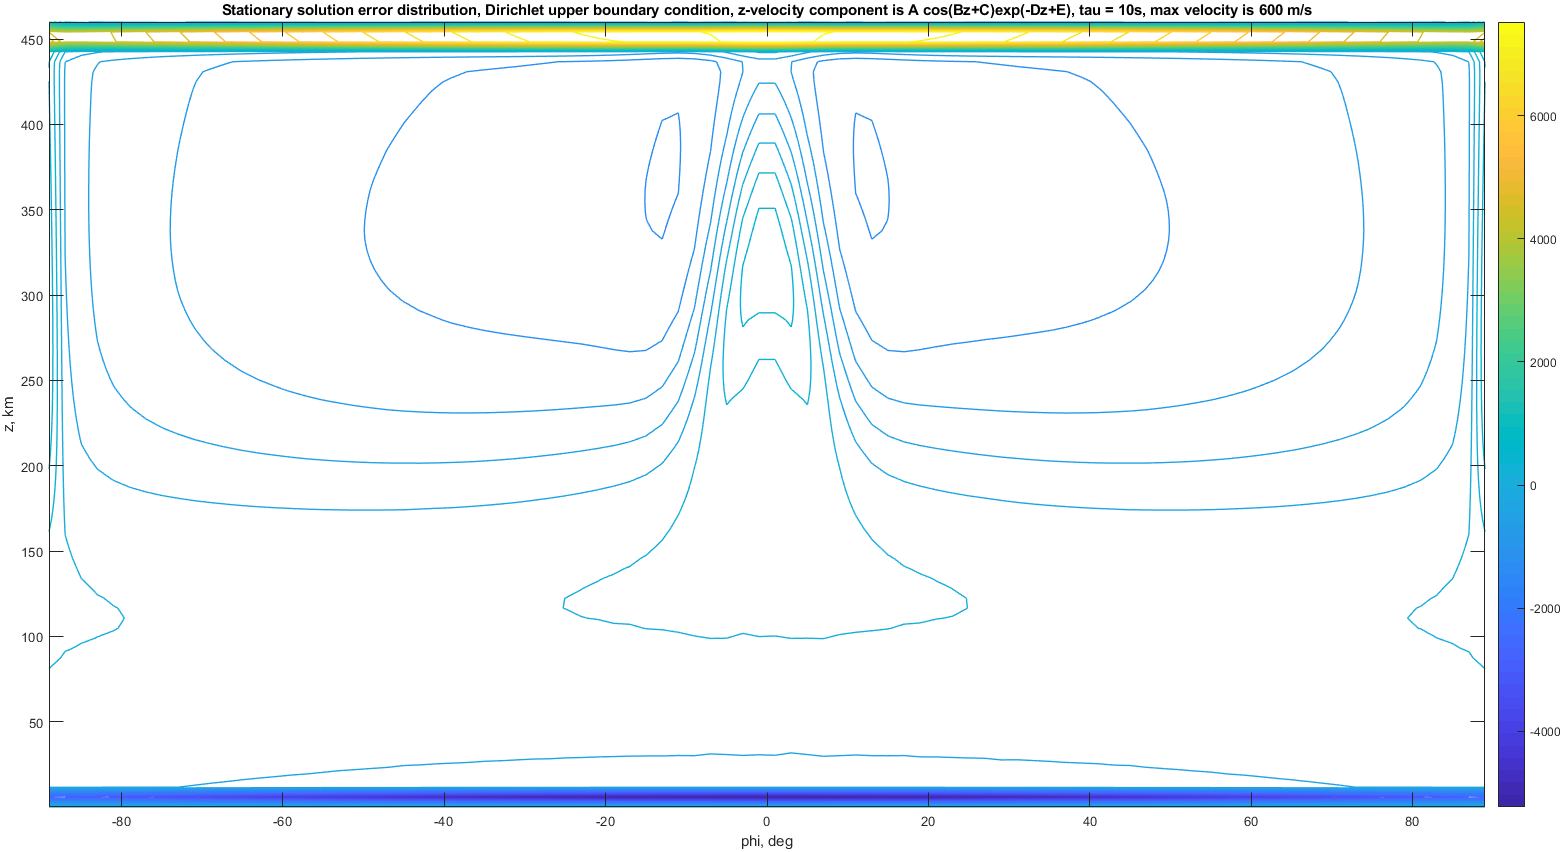
\includegraphics[scale=0.4]{cosexp_30s_vel_600}}

(а) 

\end{figure}

\begin{figure}[H]
\center{
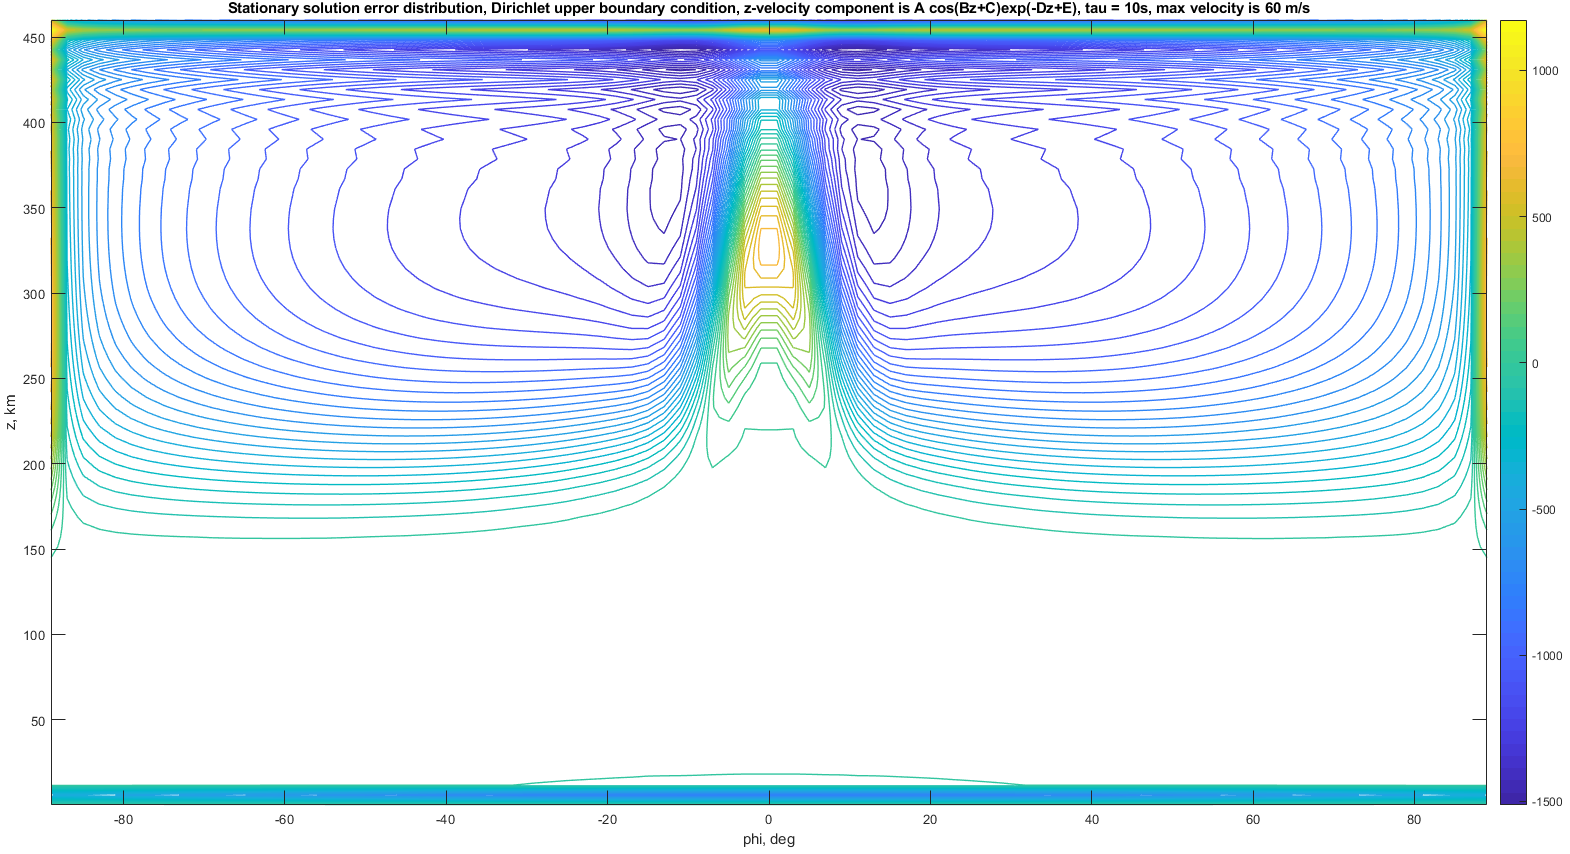
\includegraphics[scale=0.4]{cosexp_30s_vel_60}}

(б)

\end{figure}

\begin{figure}[H]
\center{
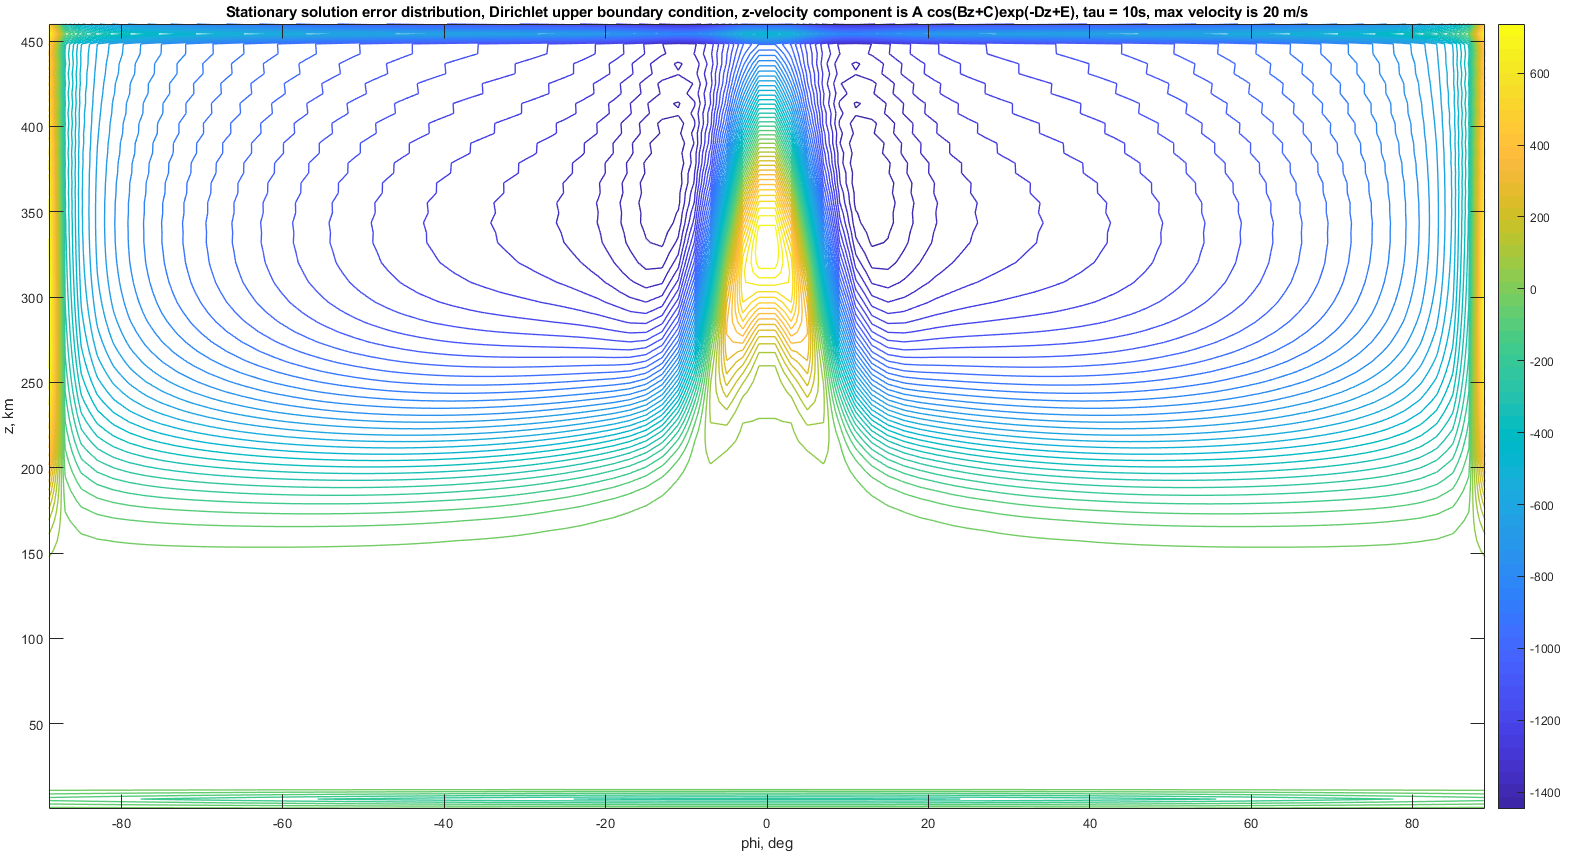
\includegraphics[scale=0.4]{cosexp_30s_vel_20}}

(в)

\caption{Широтно-высотные распределения ошибки в эксперименте по сходимости к стационарному модельному решению с переменным вертикальным полем скорости $v_z = A\cos(Bz+C)\exp(-Dz+E)$; в данном эксперименте рассматривается уменьшение амплитуды (сверху вниз соответственно $600$, $60$ и $20$ м/c); }
\end{figure}



\subsubsection{Поле $v_z = A\cos(Bz+C)\exp(-Dz+E)\exp(Fz+H)$}

Дальнейшая модификация поля скорости состоит в добавлении экспоненциального затухания также и при движении к нижней границе. Это приводит к вертикальному полю, заданному по формуле  
\begin{equation}\label{cosexp}
v_z = A\cos\left(\dfrac{z-100}{400}\pi - \dfrac{\pi}{2}\right)\exp\left(-\dfrac{z-100}{200}\right)\exp\left(\dfrac{z-500}{200}\right),
\end{equation}
где $z$ задано в км, а константа $A$ выбиралась так, чтобы максимальное по модулю значение вертикальной компоненты скорости было равно (в различных экспериментах) соответственно $450$, $45$~м/с.



\begin{figure}[H]
\center{
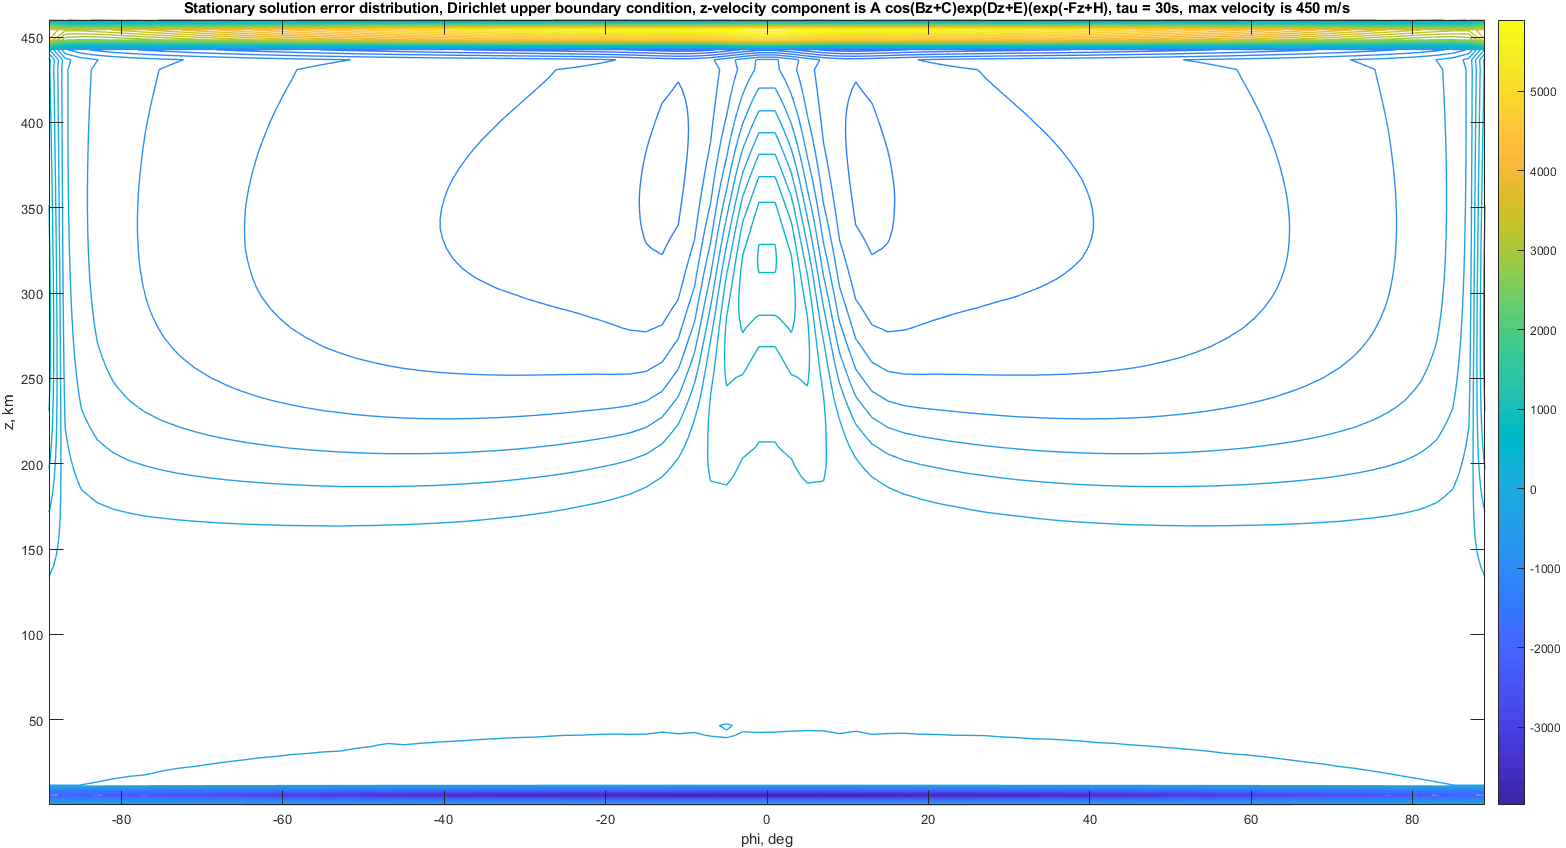
\includegraphics[scale=0.4]{cosexpexp_30s_100k}}

(а)

\end{figure}

\begin{figure}[H]
\center{
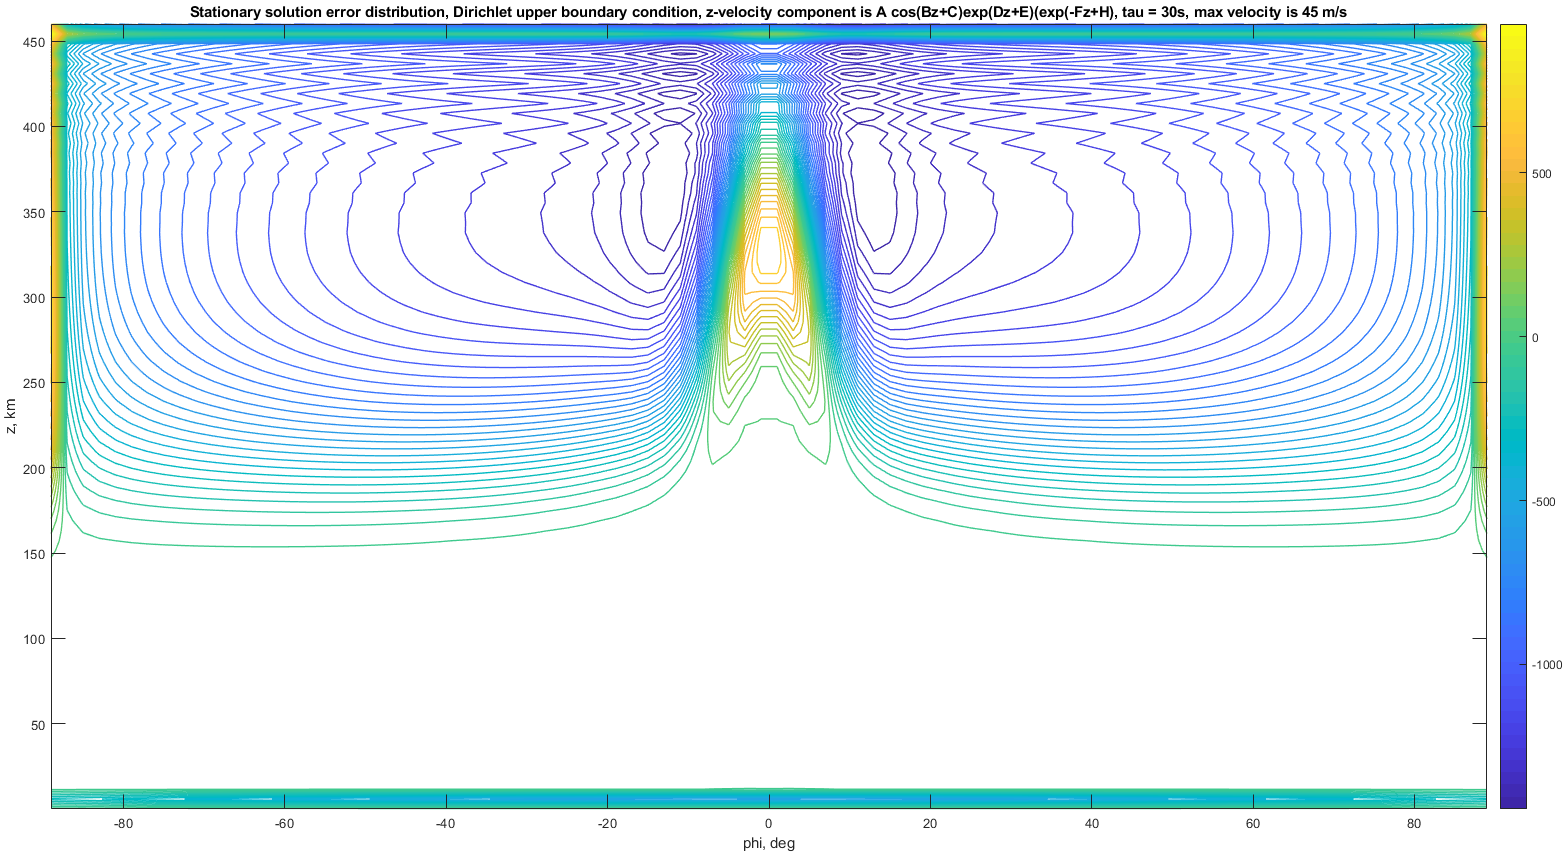
\includegraphics[scale=0.4]{cosexpexp_30s_10k}}

(б)


\caption{Широтно-высотное распределение ошибки в эксперименте по сходимости к стационарному модельному решению с переменным вертикальным полем скорости  ; максимальное значение вертикальной скорости $450$ м/c (сверху) и $45$~м/с (снизу), шаг по времени $30$ с; }
\end{figure}

\newpage

\section{Заключение}
\sectionmark{Заключение}

В работе рассмотрены основные физические процессы, влияющие на формирование поля концентрации свободных электронгов в F слое земной ионосферы, получены уравнения, описывающие динамику электронной концентрации, включающие в себя описание плазмохимических процессов, амбиполярной диффузии, переноса нейтральным ветром и электромагнитного дрейфа.

Для решения основного уравнения модели после перехода в сферическую систему координат в приближении тонкого сферического слоя использован метод расщепления по физическим процессам: к первому этапу расщепления отнесена амбиполярная диффузия  и плазмохимия, а ко второму~---~адвекция. При этом отдельная двумерная подзадача, включающая только амбиполярную диффузию и плазмохимию, детально рассмотрена в качестве самостоятельной модели.

Для двумерной модели амбиполярной диффузии разработана и применена аппроксимация смешанных производных и верхнего граничного условия потокового типа, учитывающая различные возможные знаки коэффициентов при смешанных производных и направления магнитных силовых линий. Проведено подробное сравнение двух предложенных способов аппроксимации по времени: в первом используется расщепление по физическим процессам и геометрическим направлениям, а во втором задача решается полностью неявно. При этом в первом случае за счет использования скалярных прогонок и полунеявной схемы достигается высокая эффективность расчетов, но применение расщепления снижает точность получаемых численных решений. Во втором случае для обращения возникающих матриц применяется стабилизированный метод бисопряженных градиентов, при этом выше оказываются как точность численного метода, так и время, затрачиваемое на итерационное обращение матриц.

Разработана и реализована также трёхмерная модель F слоя земной ионосферы в приближении амбиполярной диффузии со включением переноса нейтральным ветром. Для решения трёхмерного уравнения переноса использована модификация схемы <<кабаре>> на сферическом слое с нелинейной коррекцией, обладающая свойствами консервативности и монотонности, а также имеющая второй порядок аппроксимации по пространству.

Для обеих версий модели (со включением трёхмерного переноса и без рассмотрения этой части оператора) детально исследована точность используемых разностных схем: для этого использовано модельное аналитическое решение, отражающее характерные черты реального решения (резкий рост с высотой вблизи нижней границы до максимума F слоя, экспоненциальный спад выше максимума, связанный с преобладанием диффузии, в широтном направлении~---~максимум распределения в экваториальной области). Рассмотрены возникающие широтно-высотные распределения ошибки вычисления дневных стационарных распределений в модельной задаче, в случае двумерной модели получены оценки на ошибки численного решения с расщеплением и без, а в трёхмерной модели рассмотрены различные распределения ошибок при использовании различных полей скорости. При этом в последнем случае возникающие ошибки имеют характерный вид и порядок величины, близкий к ошибке пространственной аппроксимации, полученной для двумерной модели в случае полностью неявной схемы. Модель тестировалась в том числе с существенно завышенными скоростями адвекции, показав высокую точность, не превышающую соответствующий порядок величины ошибки в модели без адвекции.

В реальной задаче исследованы чувствительности получающихся высотных профилей к изменениям различных параметров, входящих в уравнение модели, а также построен вариант модели, включающий суточный ход. При этом фотоионизация задаётся зависящей от зенитного угла Солнца, меняющегося со временем.


\newpage
\addcontentsline{toc}{section}{Список использованных источников}

\begin{thebibliography}{00}
\bibitem{KulyaminDyminkov1}
\textit{Kulyamin D. V. and Dymnikov V. P.} A three-dimensional model of general thermospheric circulation. // Russian Journal of Numerical Analysis and Mathematical Modelling. --- 2013. --- 28(4). --- С. 353-380.
\bibitem{KulyaminDymnikov2}
\textit{Кулямин Д.~В., Дымников В.~П.} Моделирование климата нижней ионосферы. // Известия Российской академии наук. Физика атмосферы и океана. --- 2015. --- Т. 51(3). --- С. 317–337.
\bibitem{Schunk}
\textit{Schunk R.W., Nagy A.F.} IONOSPHERES Physics, Plasma Physics, and Chemistry. --- New York, United States: Cambridge University Press, 2009. --- 628 p.
\bibitem{Kholodov}
\textit{Холодов А.~С., Холодов Я.~А.} О критериях монотонности разностных схем для уравнений гиперболического типа. // Журнал вычислительной математики и математической физики. --- 2006. --- Т. 46, № 9. --- C. 1560-1588.
\bibitem{Fedorenko}
\textit{Федоренко Р.~П.} Введение в вычислительную физику: Учебное пособие для вузов / Под ред. А.~И. Лобанова. --- 2-е изд., испр. и доп. --- Долгопрудный: Издательский Дом <<Интеллект>>, 2008. --- 504 c.
\bibitem{Kalitkin}
\textit{Калиткин Н.~Н.} Численные методы: учеб. пособие. --- 2-е изд., исправленное. --- СПб.: БХВ-Петербург, 2014. --- 592 с.
\end{thebibliography}

\end{document}